\documentclass[]{usiinfbachelorproject}
\usepackage{subfigure}
\usepackage{float}
\usepackage{hyperref}


\author{Marco Bedulli}

\title{CSI:Cube8}
\subtitle{Augmenting Software System Representation with Corollary Information}
\versiondate{\today}

\captionsetup{labelfont={bf}}


\begin{committee}
%With more than 1 advisor an error is raised...: only 1 advisor is allowed!
\advisor[Universit\`a della Svizzera Italiana, Switzerland]{Prof.}{Michele}{Lanza}
%You can comment out  these lines if you don't have any assistant
\assistant[Universit\`a della Svizzera Italiana, Switzerland]{Phd.}{Luca}{Ponzanelli}
%\assistant[Universit\`a della Svizzera Italiana, Switzerland]{Dot.}{Andrea}{Mocci}

\end{committee}

\abstract {
The information not strictly related to a software system, likes forum discussions and code documentation, can be useful to understand how much knowledge is available about the source code. Using an augmented city metaphor as visualisation method we allow the developer to evaluate the information coverage. A developer is thus able to visualise which part needs more documentation and also directly access the online information related to it.
}

\begin{document}
\maketitle

\tableofcontents 


\pagebreak
\listoffigures

\pagebreak

%%%%%%%%%%%%%%%%%%%%%%%%%
\section{Introduction} \label{introduction}

The main purpose of this paper is offering to anyone a way to get an impression at first glance about the information coverage of a software in an immediate and intuitively way. It can be seen as the combination of the needs to get a better understanding of the backbones in a project and the needs to find all the available information related to it rendered in a easy and fast system.

Since the web community has plenty of features questions and answers on a wide range of topics in computer programming, having a pre-built application able to show the most popular discussion tightly focused on a specific problem could undoubtedly reduce the amount of time spent on learning all the functionality of the project.



\subsection{City metaphor as visualisation method } 


The city is create using a mix of information related and not to the code that are mapped to construct the building of the city.
The use of a metaphor from the physical world is the key point that makes this system particularly intuitive and effective. In fact, it allows the viewer to transfer existing perceptual abilities to the comprehension of the visualisation.\\
R. P. Gabriel \cite{gabry} said that "Habitability is the characteristic of source code that enables programmer, code ,bag-fixer, and people coming to the code later in life to understand his construction and his intentions[..]". 
\begin{figure}[h]
	\centering
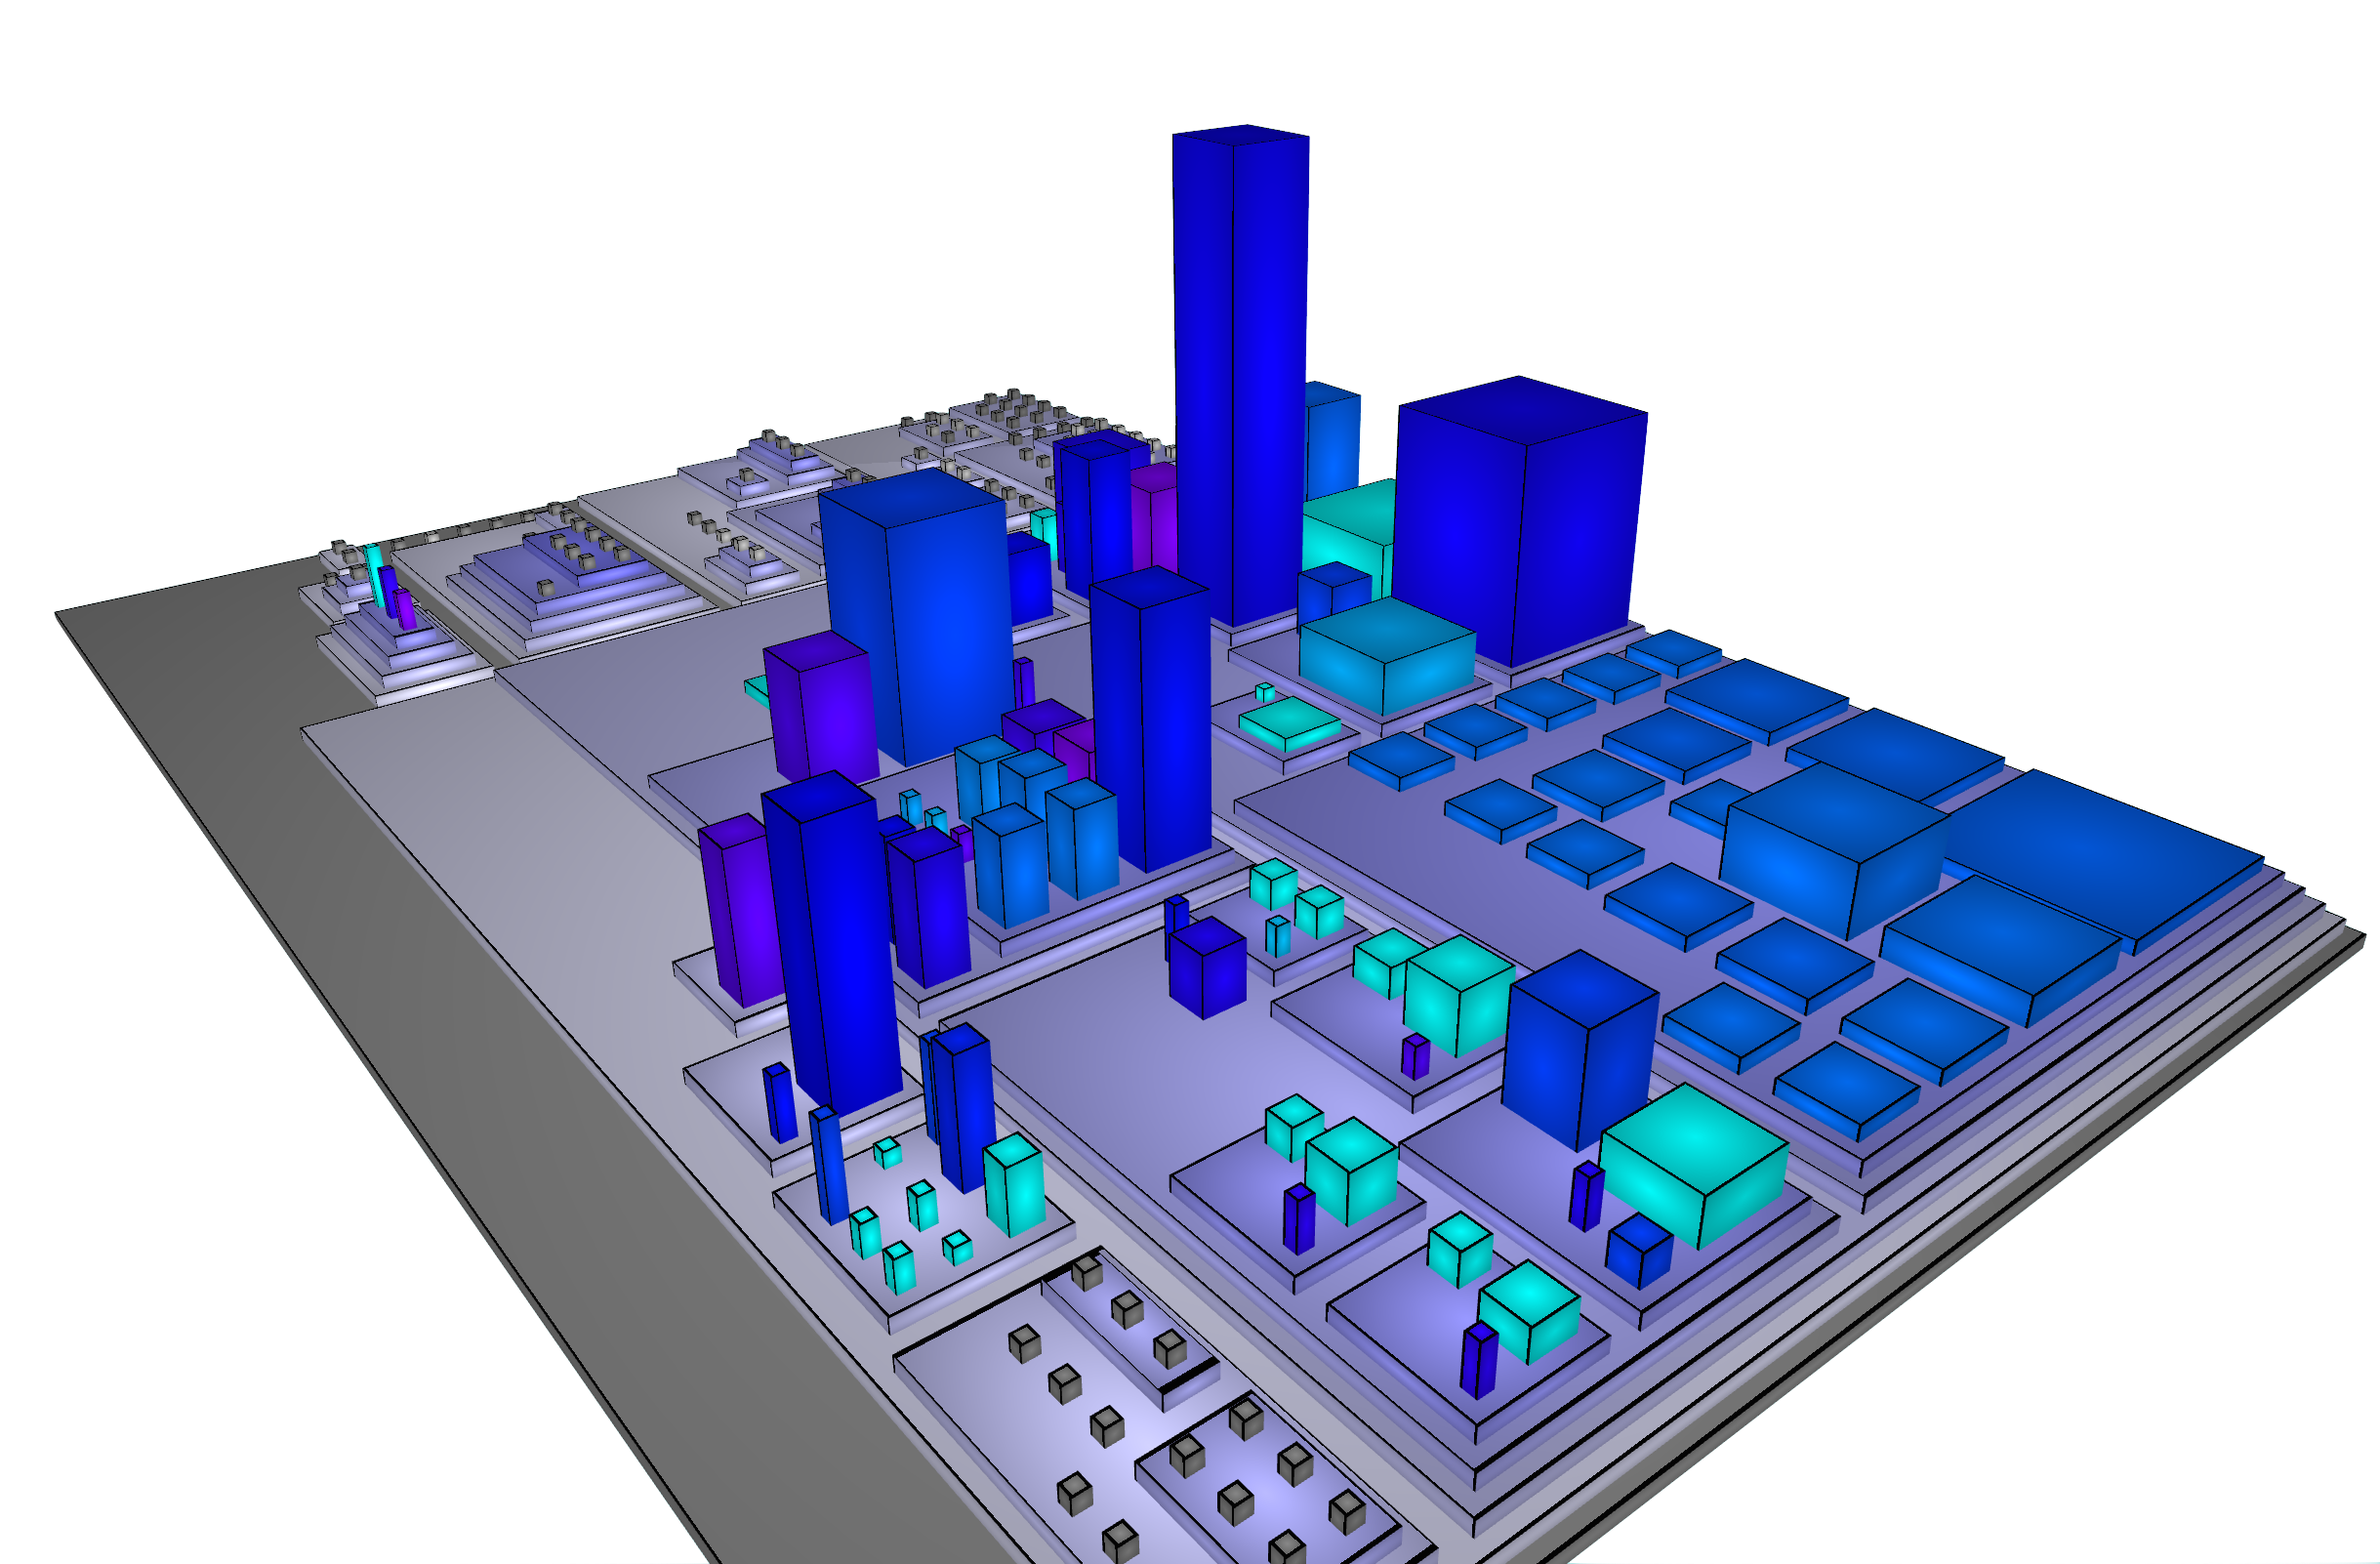
\includegraphics[width=8cm]{images/city1}
\label {myO}
\caption{A first example of a city}
\end{figure}

Starting from this concept, we use this idea of habitability as explained in \cite{vssac} Visualising Software System as City, where this metaphor is used as a way to allows the developers to get a better understanding of a specific software. \\
As main aim, we thought to help all the people that, coming to the code late during its implementation and development, need to by filled in quickly about all the reference and the information available on it.\\
By doing that, the user can navigate and interact with all the city's components, from the folder (shown as the basement in the render) to all the file that compose the project (shown as building in the render). 


\subsection{Corollary Information} 
The concept of corollary as many other concept in computer science, come from math.
Proposition B is a corollary of proposition A if B can be readily deduced from A or is self-evident from its proof, but the meaning of readily or self-evident varies depending upon the author and context. The importance of the corollary is often considered secondary to that of the initial theorem; B is unlikely to be termed a corollary if its mathematical consequences are as significant as those of A. Sometimes a corollary has a proof that explains the derivation; sometimes the derivation is considered self-evident. \cite{wikiCory}\\
In computer science we can adapt this definition: first the theorem became our source code, because is the span of our research interest.
The corollary can be self-evident if they doesn't need computation to be extracted  like the code documentation and we have also information that we  can be readily deduced from the code by doing some computation like external resources related to the code.\\

For instance, the number of class or the Interface in a file, are information that modifies the structure of the whole project because they are the fiscal parts that compose the source code; so they all may be not considered corollary information but part of the code related information,our theorem. \\
Instead, the documentation, either internal or external, has not influenced on the result of a project: the structure and the result of your software must not change by adding this information and they may reduce the complexity to implement it.
In other words, we can refer to the fiscal part of a project or the code related information  to all the information that affect the structure of the system. 
The java doc can be used as a simple example of Corollary information  because it is not important for the design proposed, but is extremely useful to understand what the code does. We could also think about the information that is not present, but could be found by using your code. Those information integrate the already existent information and gives to the developer a better view to understand more easily the entire system.

\subsection{Importance of code related information} 
We can't remove the information related to the code during the visualisation process because they give as an intuitively way to understand the topology of the project.
They are also useful to get a metric units to better understand what the information coverage means.\\ It's cool to know how much java doc you have respect to a file, but if you don't know the characteristics of that file, you can't say if the documentation is enough or not. Is also useful to use the purely code relation information to have a main idea about the struct of the system, as we will see later, where we analyse a system, we are using also information strictly related to the code to get some code disharmony.

\subsection{Document Structure} 
In section 2 we present the related work. We are going to analyse the functionality of system like Cube8 and we explain briefly how stormed works since is use in this project.
Then we explain the approach used and the different metrics that we used in section 3.
In section 4 we show  two different projects and how to use our system and which kind of informations are possible to retrieves.
Finally we conclude with some improvement that will be interesting  to be implemented.


\newpage


  
\section{Related Works} \label{related works}
Cube8 is a mix of two different sectors and works. One is the visualisation method for a software system and the other one is the way to get the corollary information.\\

\subsection{Program Comprehension through Software Habitability}
Program Comprehension through Software Habitability \cite{programComp} propose a city metaphor in which there are a fix number  of building type such as Skyscraper, Office building, Apartment Block,mansion and House. They propose two mapping: Boxplot-based Mapping and Threshold-based Mapping. Also they using a box-packing algorithm to visualise the city.  We are using the same idea of box-packing to organise the city. We also apply the same city metaphor: classes are representing as building located in city districts which in turn represent packages. \\The colour meaning is completely different since we have to visualise different information. In those paper they are concentrate about the structure of a software, here we would like to visualise the coverage information. We still allows the developer to get an idea about other software propriety like classes and interface distribution, system identity disharmonies by  applying different metrics in a dynamic context. The size of the building are code dependent, this allows a better understanding about the system. 

\subsection{Visualise Software system as Cities}
Visualise Software system as Cities \cite{vssac} is also propose a 3d environment in which the software system is represent as a city, whit different class of buildings. It's also implements a way to navigate and interact with the system.is possible to select any artefact and interact with them, spawning complementary views,  a tagging system and a query system.
In Cube8 we have only some of this feature like a basic query system that allows to search for  file name and perform different actions. Is also possible to read the code and navigate through the information found on the web related to a particular building.\\ \\

\subsection{StORMeD}
The StORMeD \cite{stormy} gives a dataset of JSON files, one for each discussion that contain an H-AST about the discussions. The discussion parsing happens in two different step:the former consist into  HTML tag rules to extract the information unit. The latter concern the effective use of the  heterogeneous island grammar.This approach is an extension of Bacchelli \cite{Bacchelli}.  
We are using simply this dataset to compute the information coverage of the system.

 




\newpage
\section{Approach} \label{approach}

\subsection{Introduction}
In this section we are going to analyse the approach used in our tool and explain why we are made same decision. The system language that we analyse is Java, so a Object Oriented language. This imply that we are going to speak about classes, interfaces methods and fields. The container, or building, are the files and not the classes so on building can have more classes and interfaces.

\subsection{Information Strictly related to the code}
As describe in the introduction we are used code related information to give to the user a better understanding about the locality of the code. To demonstrate this concept you can see two render about the same code. For simplicity we used a huge system that consist of two classes. ClassA has 4 methods and ClassB has 4 method and the same number of fields. We have to find which class need more documentation. The Java Doc, is express in percentage respect the number of method. The colour goes from light blue to purple: light blue represent the minimum and purple the maximum percentage of information available. In the figure \ref{fig:strictly:a} , we can see that the big box at left as full documentation, instead, the right one has less. We assign the width of the building as the fields count and the height the method count;therefore the purplish class is our target and is also intuitively the ClassA since is larger then the other one. \\
Suppose you have to use the figure \ref{fig:strictly:b}: where is assign to the width the number of discussion, height the number of java documentation and the colour the number of methods. There are represent  more information not related to the code at once, and has only the method count as code related information. The city become unusable since you can not determinate which is the class A and the class B since the only difference is on the number of fields! But at the same time you can made some general statement about the relationship between java documentation and discussion.\\
 Later in this chapter we are going to analyse more in detail colour system and the meaning of the used metrics.
\begin{figure}[h]
\centering
\subfigure[Mapping as Width:N of method, height: Number of field, colour: javaDoc ]{
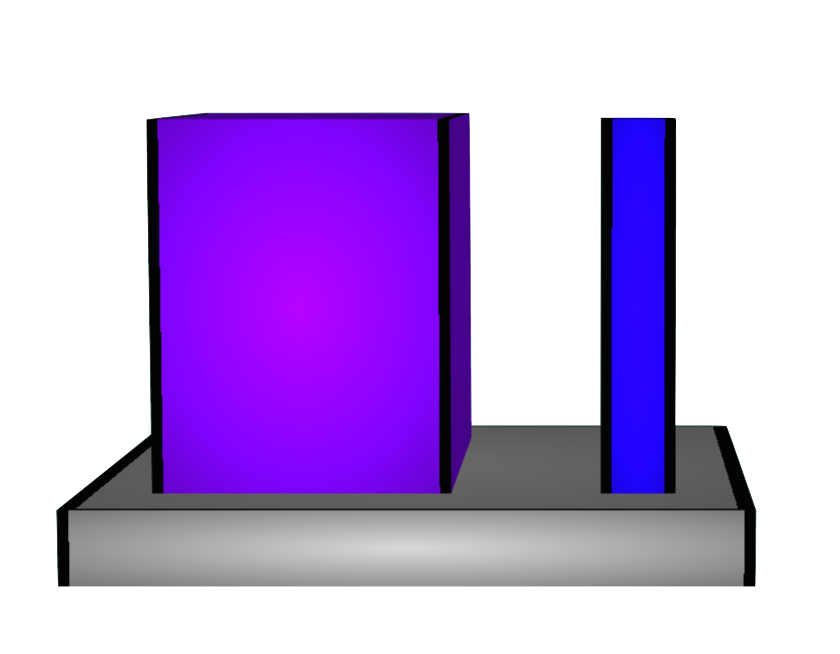
\includegraphics[width=.45\textwidth,height=4cm,keepaspectratio]{images/correctC}
\label{fig:strictly:a}
}
\hspace*{\fill}
\subfigure[Mapping as Width:Discussion count, height: Java doc, color: N of method ]{
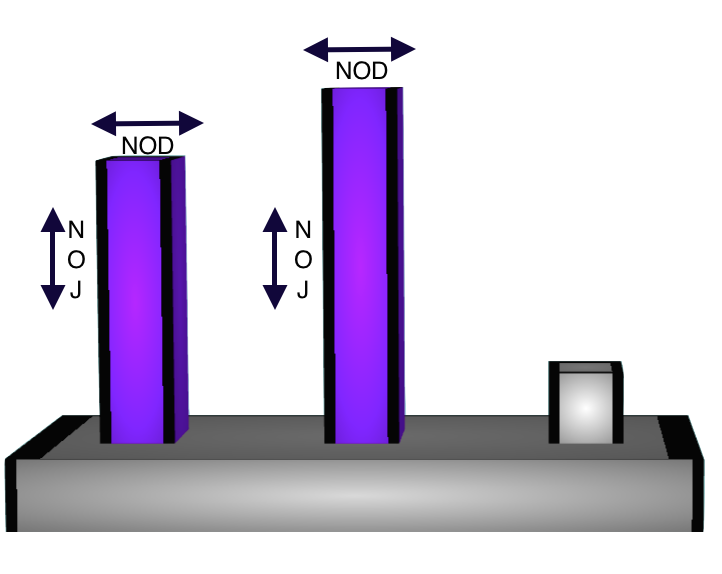
\includegraphics[width=.45\textwidth,height=4cm,keepaspectratio]{images/wrongC}
\label{fig:strictly:b}
}

\caption{Information Strictly related to the code}
\label{fig:strictly}
\end{figure}
\newpage

\subsubsection{Class and Interface}

The classes and  interface are another metrics that we add to our tools. Remember that the basic building represented is the source file.  By the Java Code Conventions \cite{oracle}  "Each Java source file contains a single public class or interface. When private classes and
interfaces are associated with a public class, you can put them in the same source file as the public class". This mean that we could have more classes in a single source file and therefore could be useful to have a metrics that give to the analyser the ability to find this relations.
Is also useful as a monitor of the level of coupling in the code. If there are a file with a huge amount of class there could be a low height degree of coupling and so the could become hard to maintain. We will see an example during the analysis of tomcat.


\begin{figure}[H]
\centering
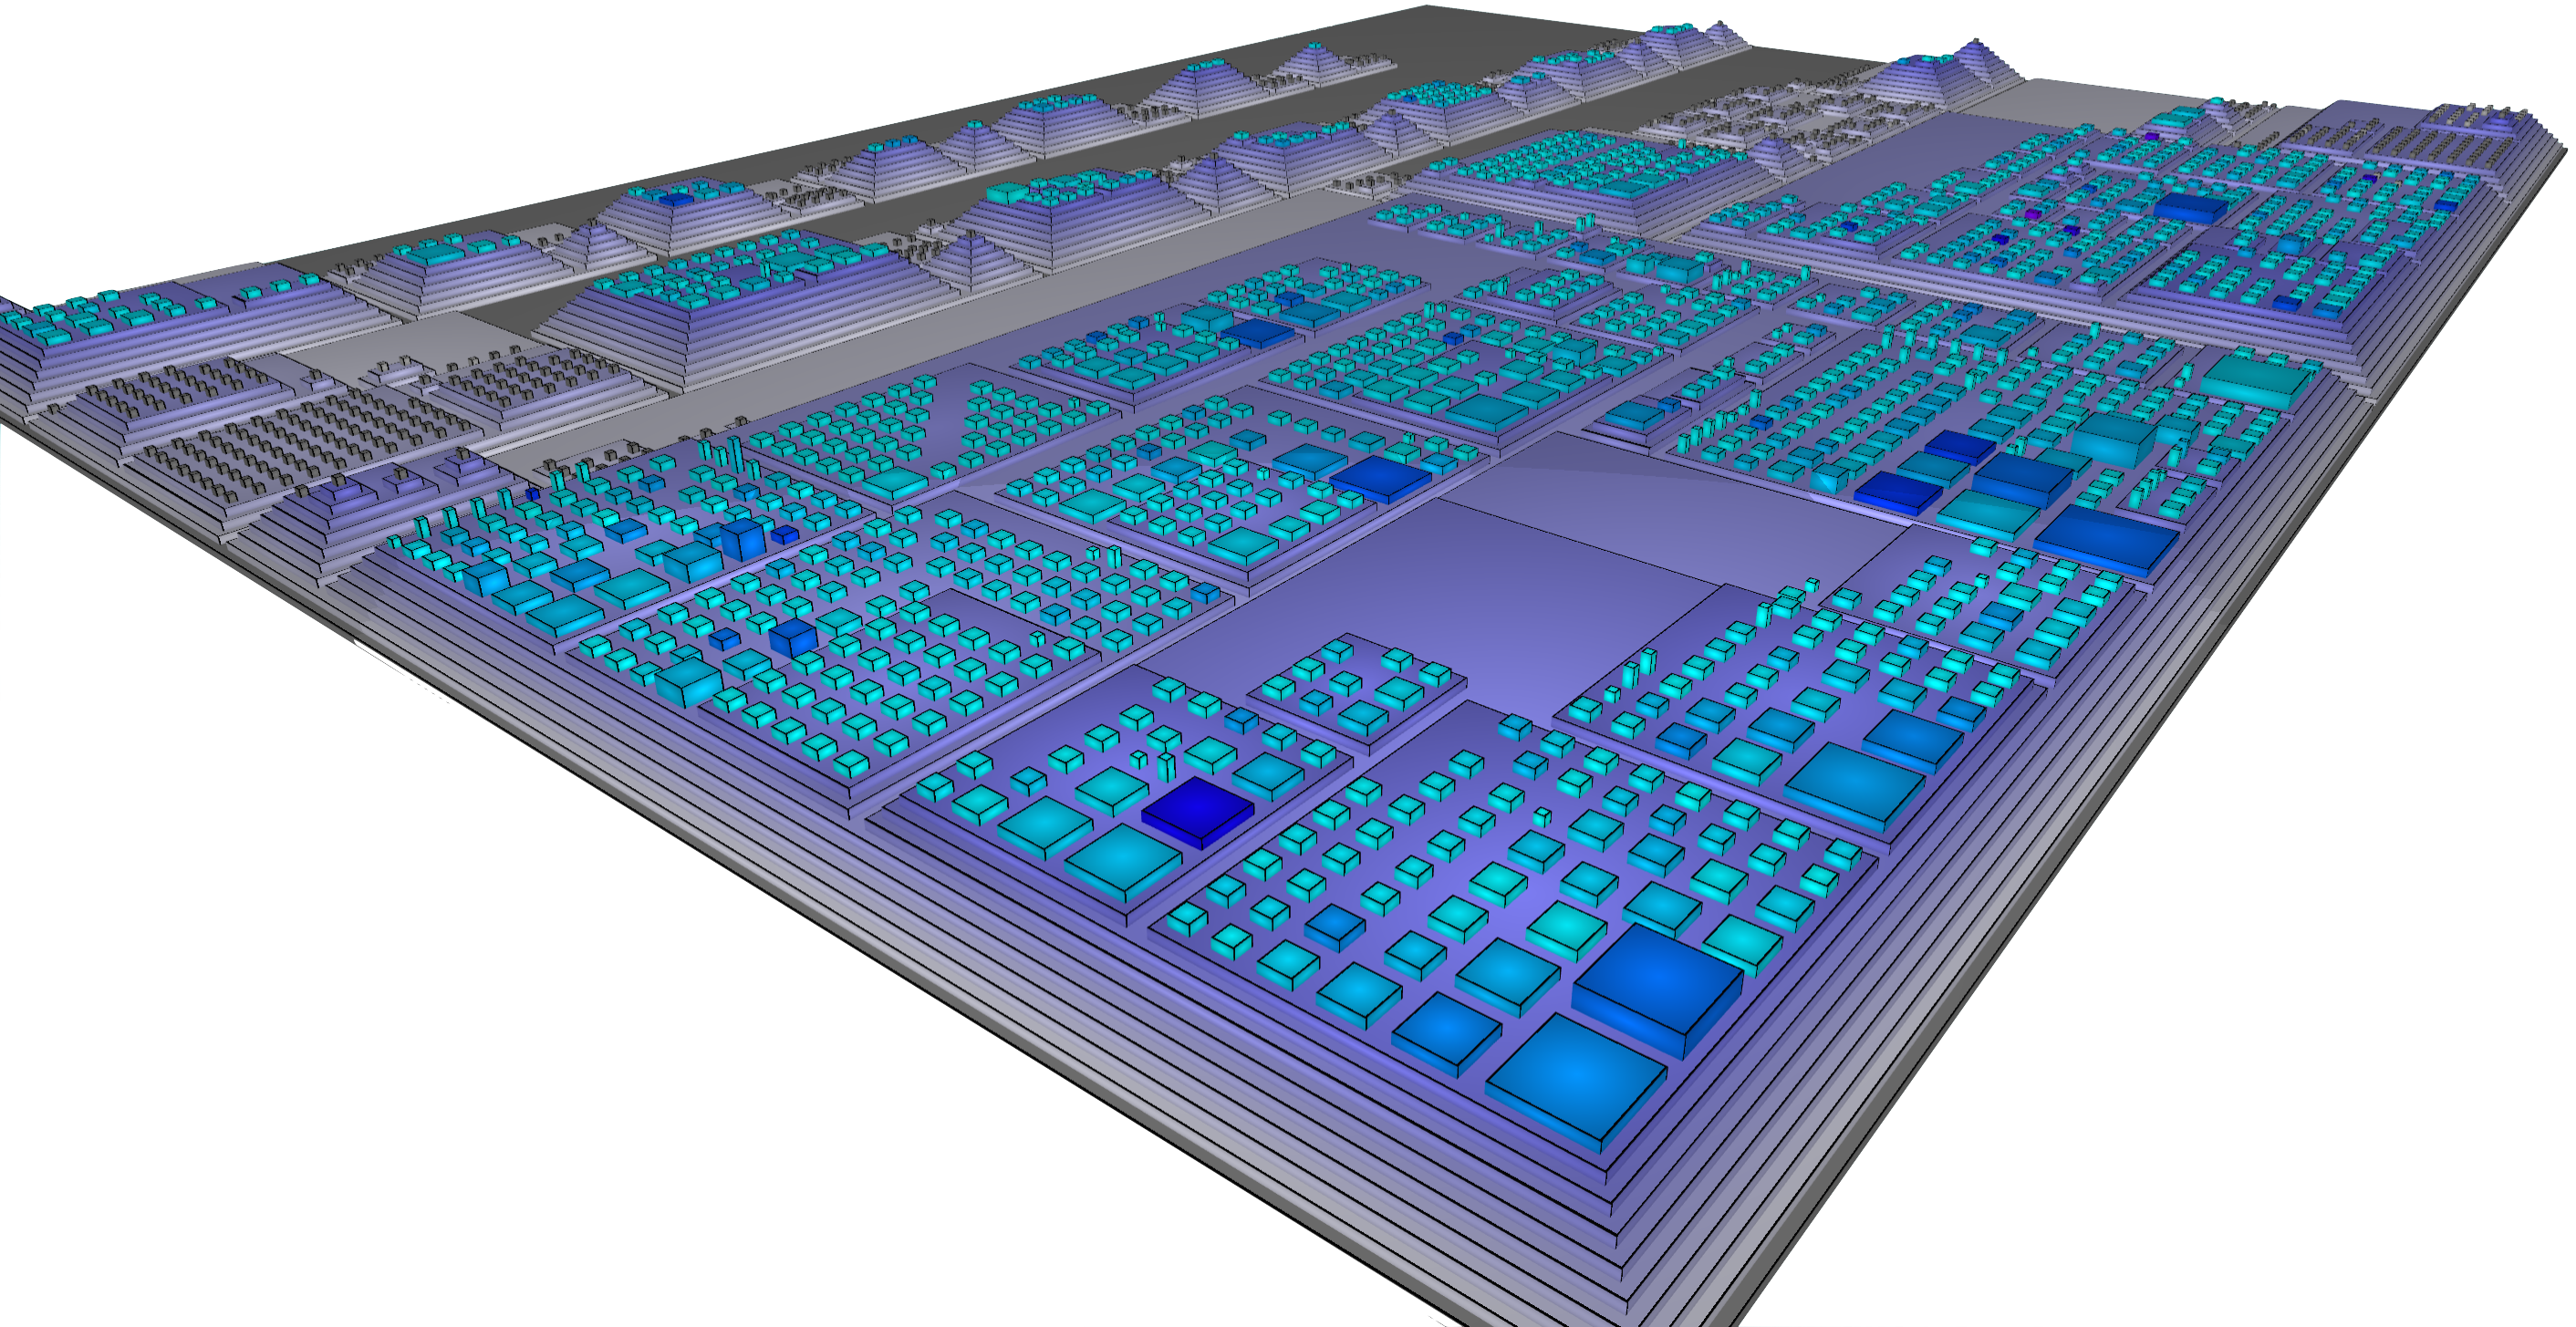
\includegraphics[width=.60\textwidth]{images/ClassesAndInterfaces}
\caption[Classes and Interfaces Mapping]{Mapping as Width:N of Class, height: Number of interface \label{fig:classInterface}
}
	
\end{figure}

This is an example, figure \ref{fig:classInterface}, where we analyse this two concept in a big project.
As you can see there are a few classes that could need some check to make sure that this design  principle is respected. We use the width to show that is possible to change metrics respect to what we are going to look at. What is also useful is to map the class to the colour,as done later. This allows to leave the same width and height of the building and is also easier to identify the class or other disharmony. 


\subsubsection{Identity Harmony	}\label{sec:idHarmony}
Design disharmonies are formalised design shortcomings to detonate pieces of system that exhibit design problem. With our tool we can only identify some of the identity harmony. Every entity in the system must justify his existence. Does it implement a specific concept or is it doing to many things or does  it nothing?\\

We can identify 3 kind of disharmonies:
\begin{itemize}

\item{God Class}:is a class that does too much . In our representation appear like a big box.
\item{Brain Class}:is a class that accumulate an excessive amount of intelligence,usually has a lot of methods: it's look like an antenna
\item{Data Class}:is a class that hold a lot of data and doesn't perform any operation:it is appear to a be a big and thin box.

\end{itemize} 


\subsubsection{Methods  and Fields}
Method and field are the main component that compose a class or an interface. In the tools, we are using this two measure to map  the size of the buildings. The reason is that this two informations gives the correct granularity to have a better understand about the system.\\
We can also identify a potential God Class that has a hight number of method  or a Data Class that has a hight number of field and a few  methods.
Let's get an example. We using the same project as before.
\begin{figure}[h]
	\centering
	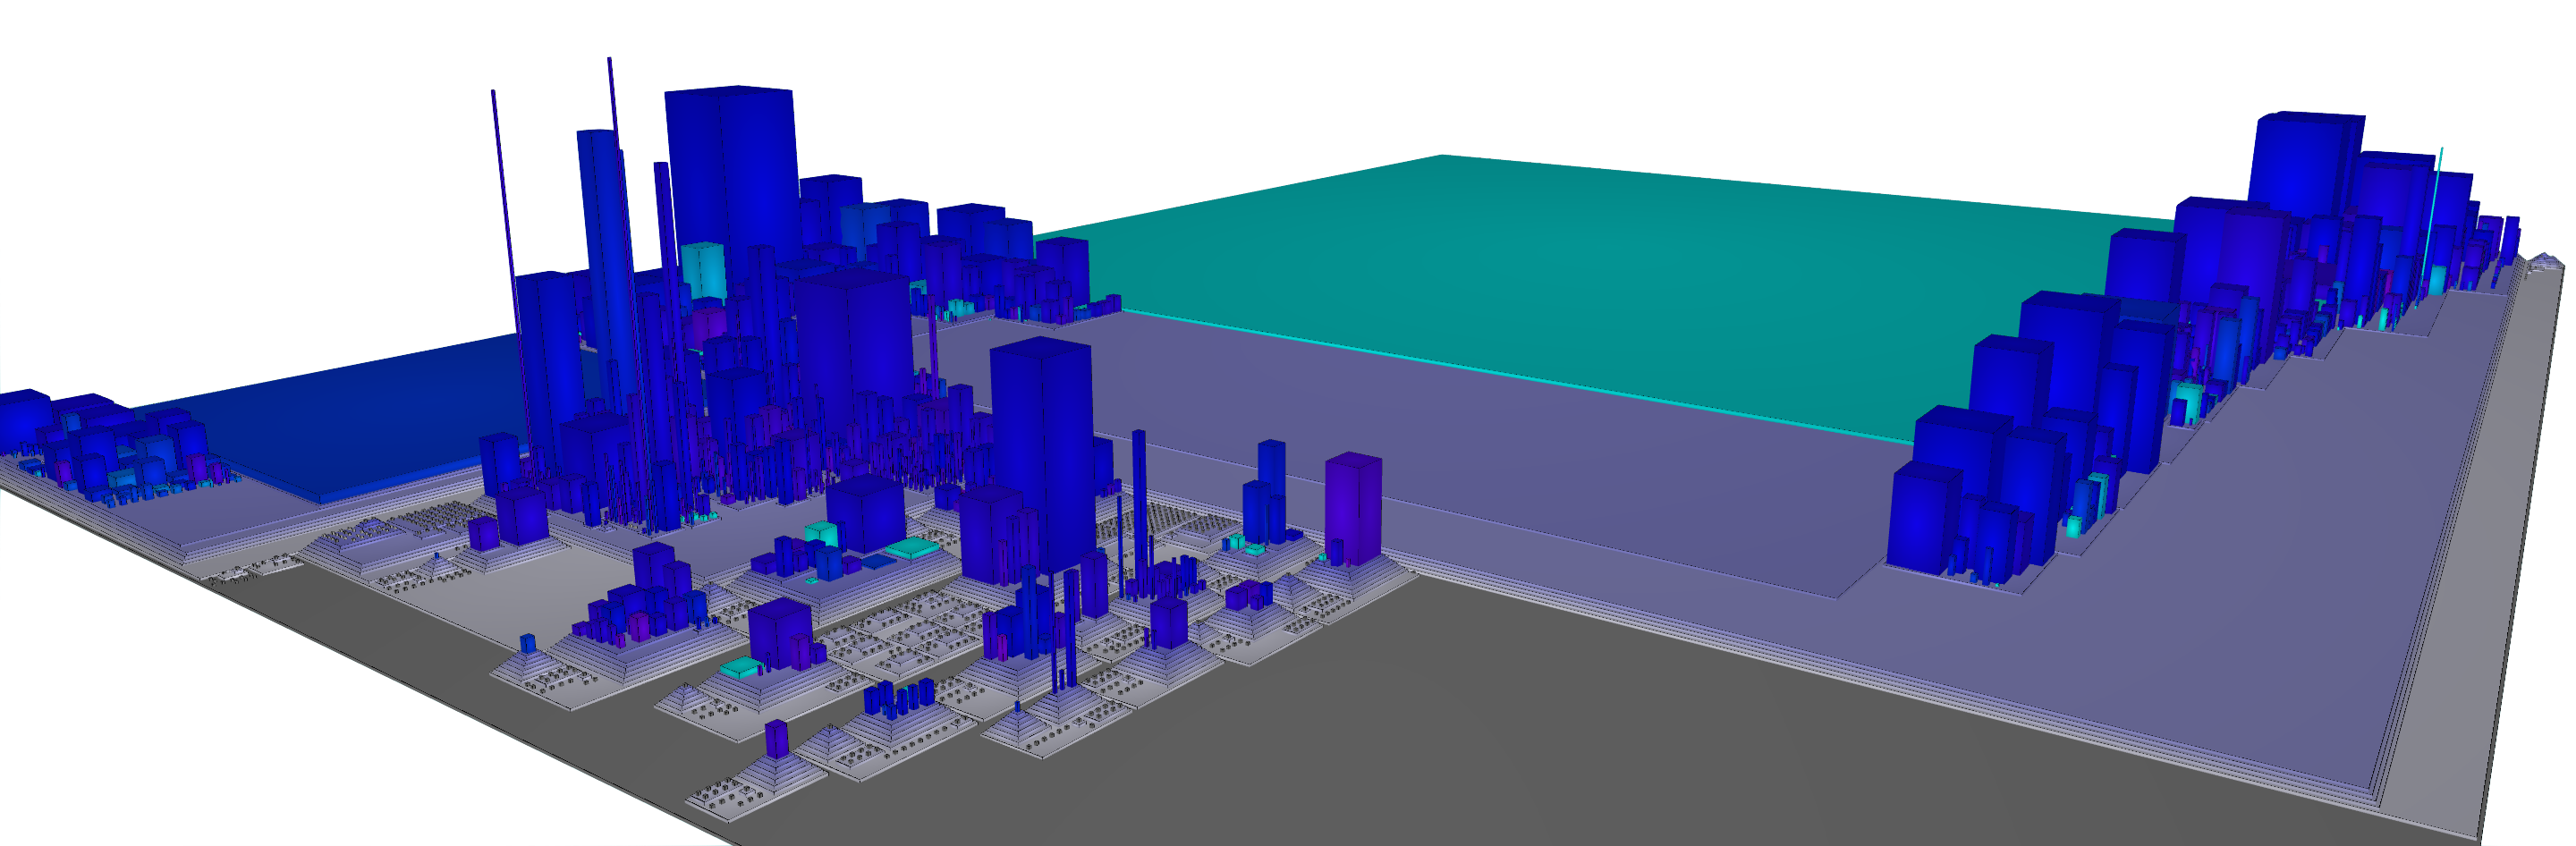
\includegraphics[width=1\textwidth]{images/fieldAndMethod}
	\caption[Fields and Methods Mapping]{Mapping as Width:N of Fields, height: Number of Method \label{fig:fieldAndMethods}}




	

\end{figure}

It's easy to see that there is a  flat an big building that could represent a Data Class and  there are two thigh and height building that could represent a God Class. In this case the both candidate for the god Class are tests. Instead the Data Class has really  686 fields.




    
\newpage
\subsection{Information Not Strictly related to the code}
The information not strictly related to  code are the core of this paper. As we sow before, there already exist tools that allows the visualisation of a system as a city, and they does a lot of computation around strict related information. What we interesting, instead, is the amount ok knowledge that are available about a given system. This knowledge are meaningful to get an idea about the complexity of understanding a software system and where it should be use more effort.At the same time it  could  be use as a monitor for the developers to understand which part of their code need more documentation.  


\subsubsection{Java Documentation}
Collecting and visualising the java documentation was the first step of the process to collecting the coverage information since it is integrated on the code and he doest require any  particular computations. It cover an important role in the process of understanding the functionality of a given code since is written directly by the developers and should be use in each method, field and class definitions.\\
With this computation unit is possible to visualise the documentation state of a project. We usually map the java documentation using the colour; it is collect only the method documentation since we claim that was a good level of granularity. The class documentation was not enough, it gives only a global view of the functionalities.

\begin{figure}[H]
	\centering
	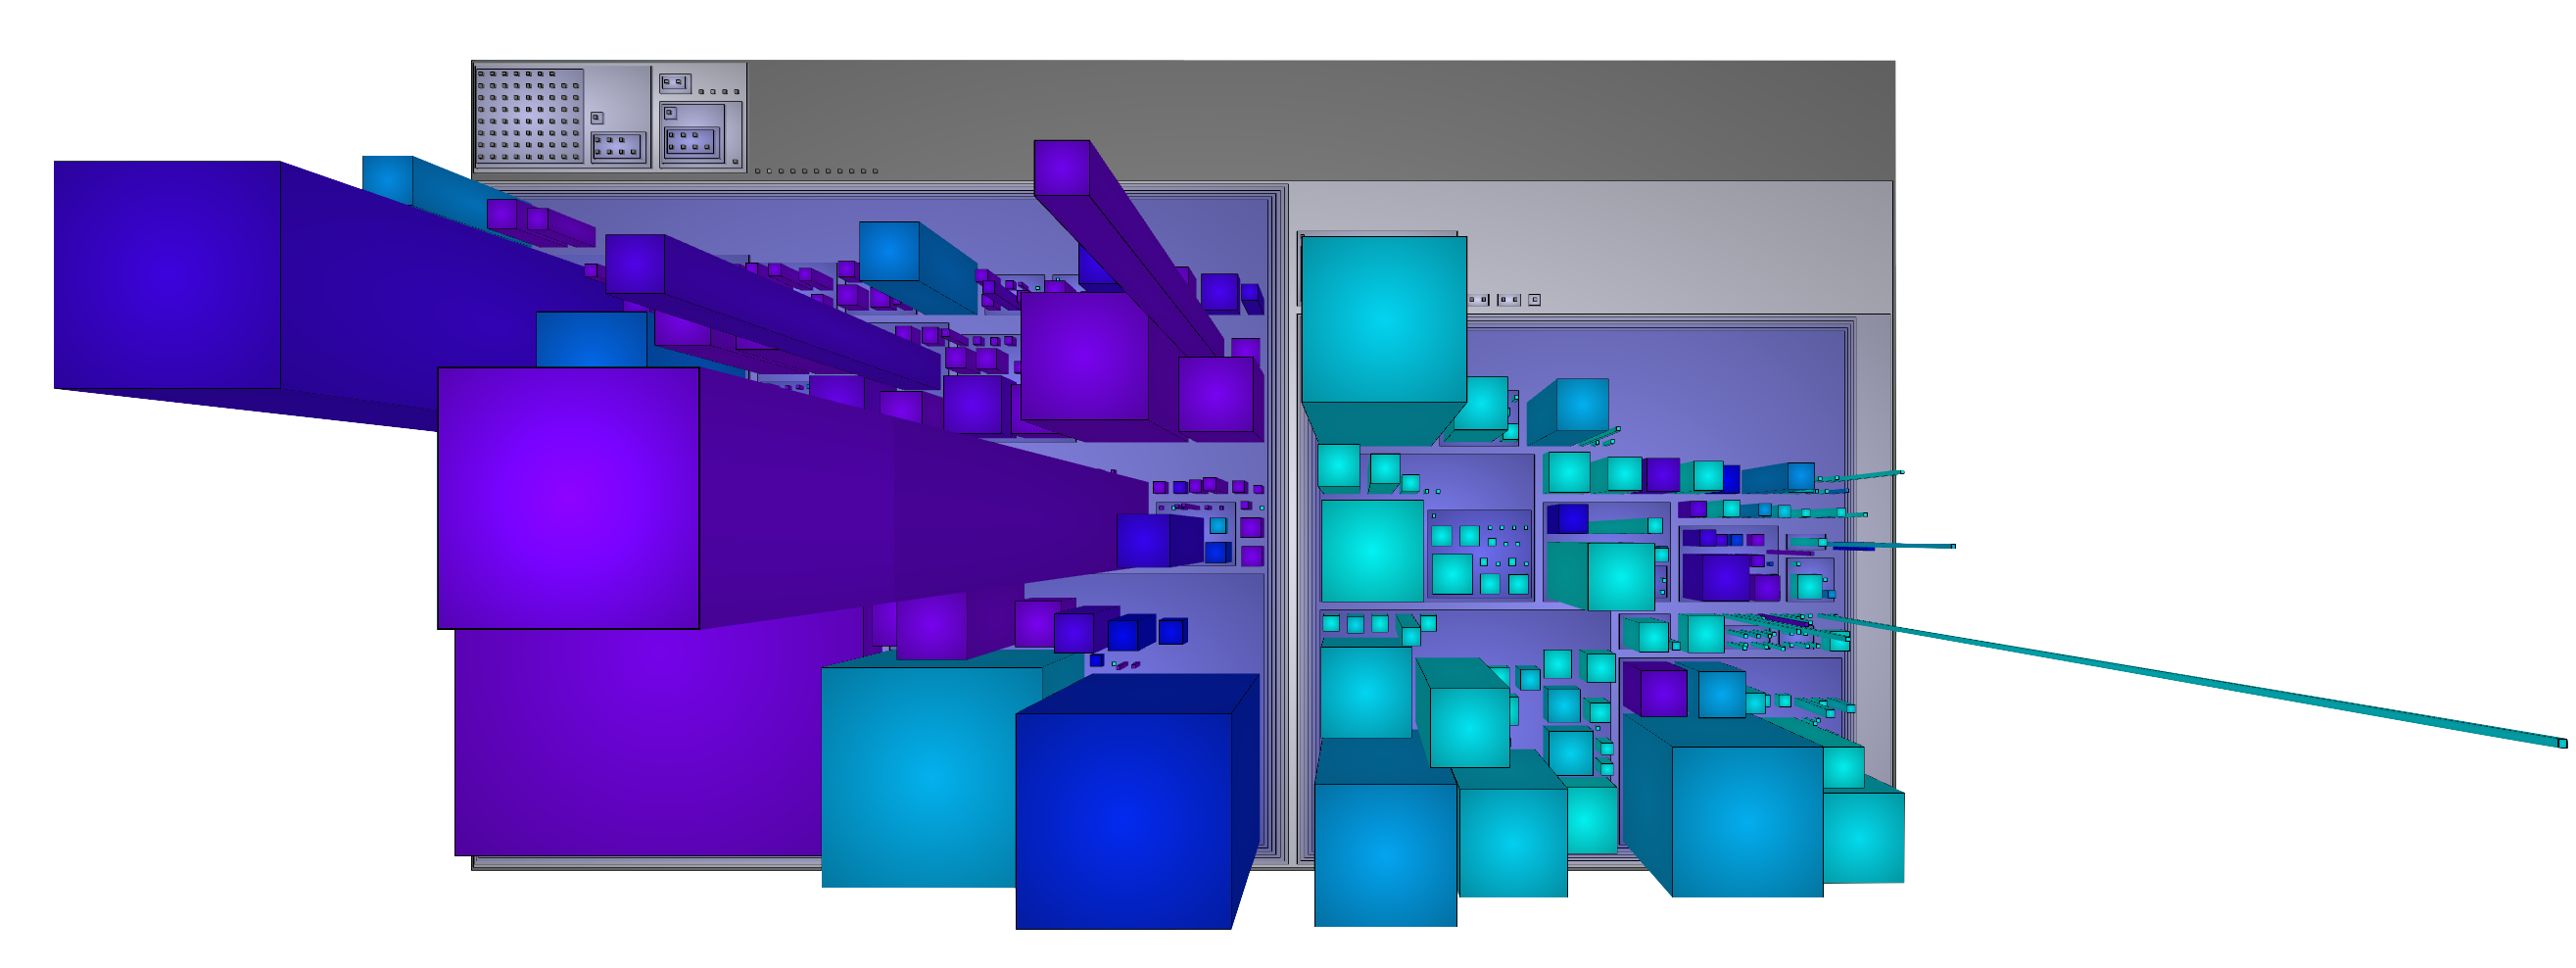
\includegraphics[width=1\textwidth]{images/javaDoc}
	
	\caption[Java Documentation Mapping]{Mapping as Width:N of Fields, height: Number of Method,Colour: Percentage of documented methods\label{fig:javaDoc}}

\end{figure}

Figure \ref{fig:javaDoc} is example of a city in which the colour represent the percentage of documented methods.The project is the apache common-lang . Is very interesting to see that half of the project has a documentation coverage greaten that the 80\% and in the other one is very rare. In reality this is a common case since a lot of project does't document the tests.\\
To help the analyser to understand the documentation coverage we also provide a package base colouring system. In which the colour of each package is the average of the child component. In  this case it look like figure \ref{fig:OnlyPackage}

\begin{figure}[H]
	\centering
	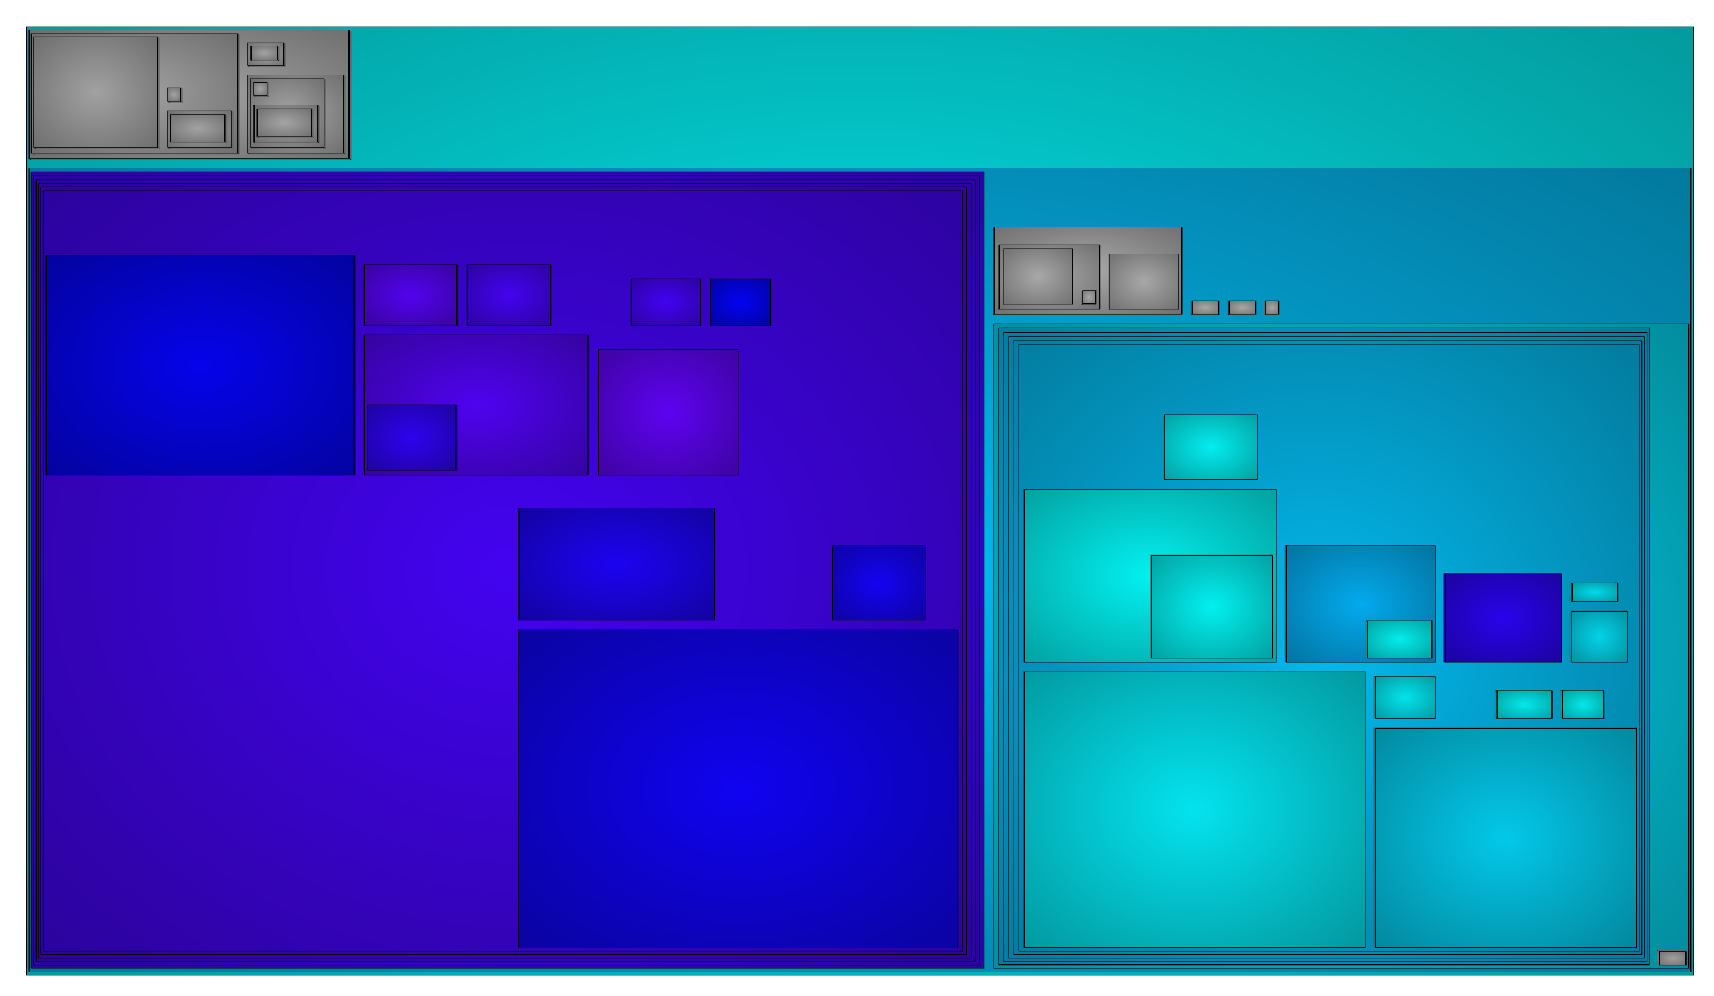
\includegraphics[width=0.5\textwidth]{images/javaDocOnlyPackage}
	
	\caption[Java Documentation Mapping Only Package]{Mapping as Width:N of Fields, height: Number of Method,Colour: Percentage of documented methods\label{fig:OnlyPackage}}
\end{figure}


\subsubsection{Stack Overflow  Discussion}
Stack Overflow is one of the most popular developer's forum. It contains a lot of code snippet and text related to the code. What we try to do using this visualisation method is to show to the user all the available discussion related to each method call. As you could observe the granularity is different respect the java doc metric. That allows to understand the complexity to read and understand the methods code not what the method itself does.We get he dataset update to august  2015. It contains ruffly 490000 discussions with more than 20000 different imports declaration and 100000 methods call.\\
In this stage we have all the repository code and all the discussion information (method call and import) from the stormed Dataset how we can merge to get a good approximation? We didn't use any type resolution system and this is a future improvement of the system. Now we are going to analyse the way that our tools match this information.
Java imports are match easily by using a string matching. We ignore the asterisk at the end of the import if is present. 
We also analyse only the external import and not the import of the system.\\
The Method is a bit more complex since we use the name of the method call and the numbers of args. In this way we have a better matching.Remember that the discussion contains code that is not complete so we have to make an approximation to retrieve the data.
The metrics that results is a sum over the total information that should be found. By interact on each building is possible to see the link to the stack overflow discussions.\\
The figure \ref{fig:disc}  is an example of the discussion found in respect to a building. The colour represent the number of discussion in absolute way. We see later what this means. As you can see there are two classes that as more discussion that the others . Of course classes that has more field are light blue coloured.

\begin{figure}[H]
	\centering
	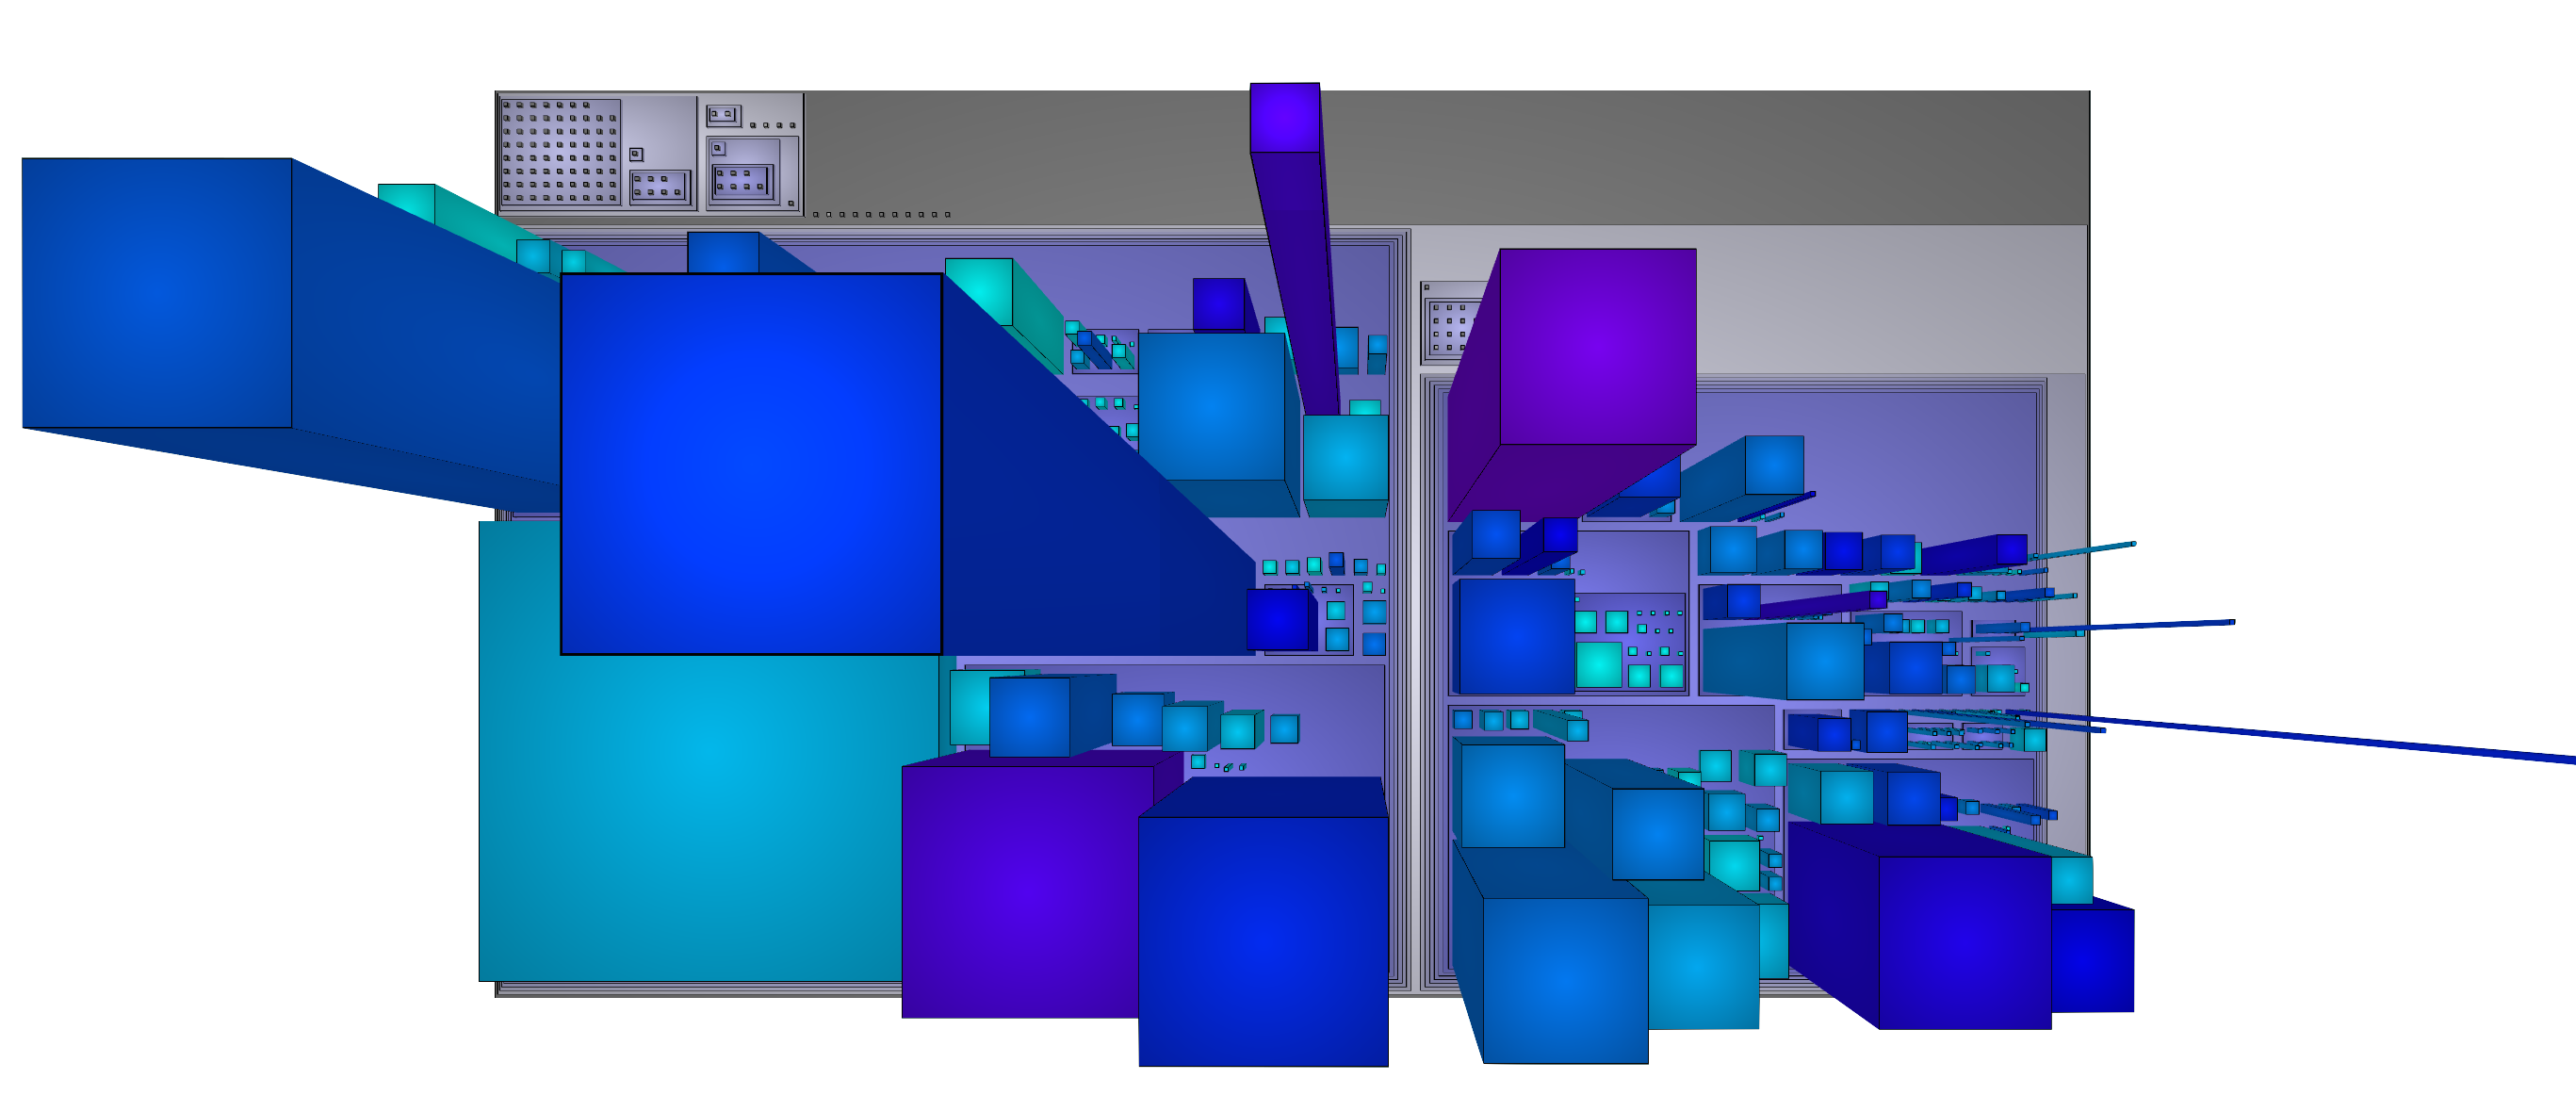
\includegraphics[width=0.8\textwidth]{images/discAbsLang}
	
	\caption[Discussion Mapping]{Mapping as Width:N of Fields, height: Number of Method,Colour: Absolute number of discussions\label{fig:disc}}

\end{figure}

In figure \ref{fig:list} you can see the list of link for each method call or import declaration:


 \begin{figure}[H]
	\centering
	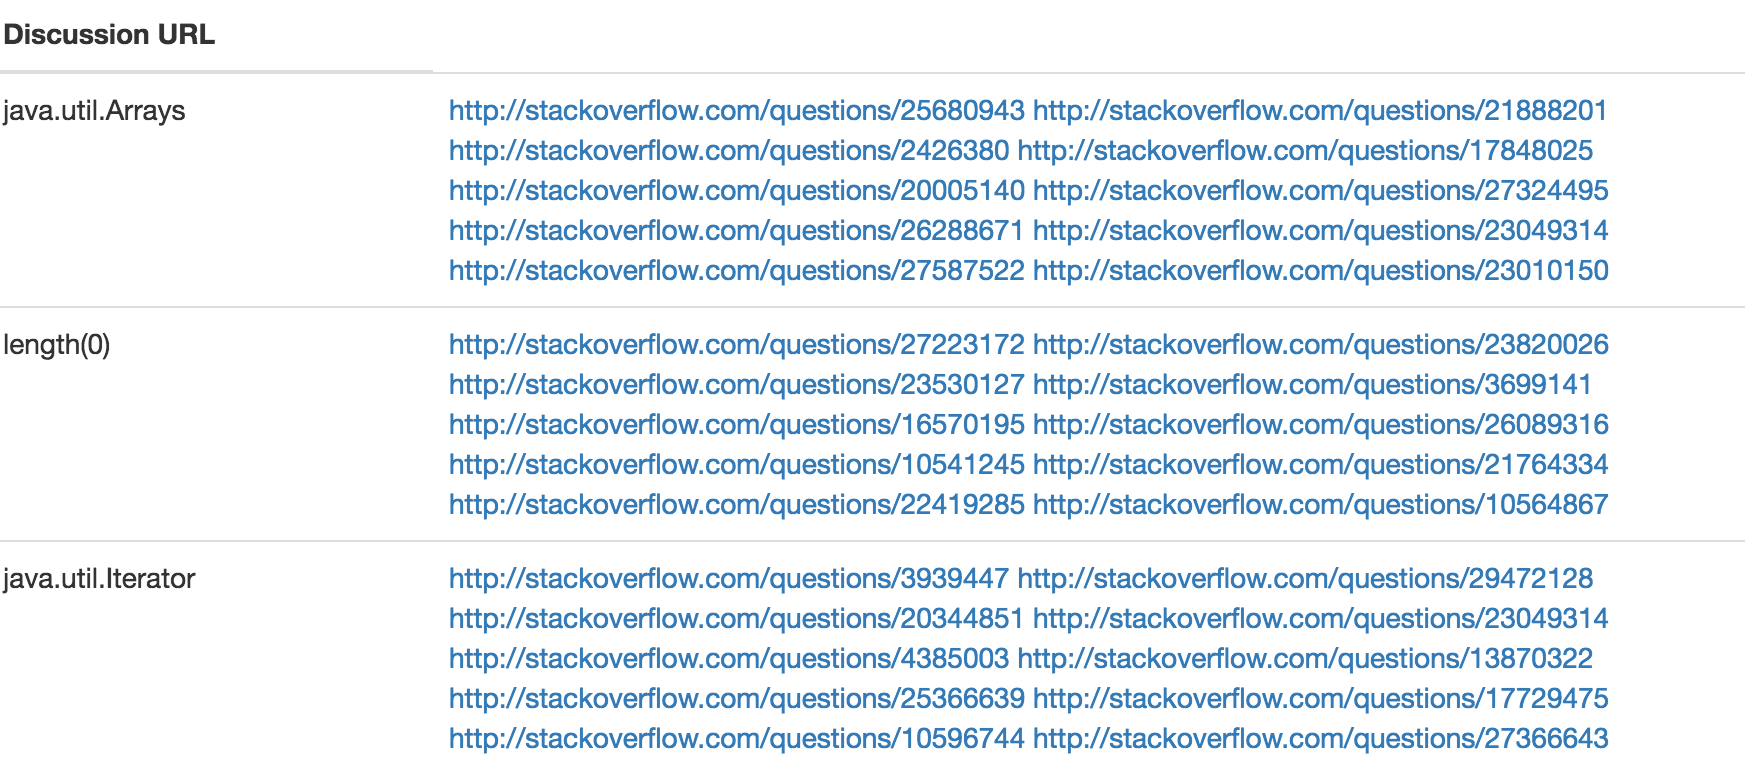
\includegraphics[width=1\textwidth]{images/listOfDiscussions}
		\caption[List Of Discussions]{List Of Discussions \label{fig:list}
}

\end{figure}


\subsection{Merge Code Related information with Corollary Information}
The Code related information helps to identify the different component of the city and also helps to found design problem over the application. The corollary information, instead gives an idea about the information coverage.How we can mix together to get a global overview of the entire system? As you can see in the picture before we are using the information related to the code to give a size of the building, and we use  the colour to represent the information coverage. In this way we improve the concept of locality, since a developer should remember a file not for the number of documented method but for the number of methods or fields.  

\subsubsection{Percentage and Absolute Numbers of informations}
The corollary information could be computed in an absolute or in percentage. In the former way we count the number of information available and is possible to see which file contains more documentations. The percentage, instead, is computed over the total amount of information that it could be found. This metric is useful to spot which files have more documentation and which are not documented. We also decide to give 0\% of documentation were we can't find anything because either are all fields or all the import are from local package.

\subsubsection{Using Java Doc and Discussion together}
To get a better understanding about the information coverage we have to mix up the documentation and the information related to code. We made an average of both since they correspond to two difference level of granularity. The java documentation refer to a method and the discussion refers to either import or method calls. We can show the result in both way: percentage and absolute.\\
In the former case, the developer can get a better understanding about the the percentage of the information available. This is useful to guess the effort require to understand a code. The latter, instead, is used to see were there are more concentration of information and where are not. It could be useful to identify package bad documented.
  



\subsection{Colors}
The colours is used to show another metrics. They goes from light blue to purple. They are very useful to give to the developer a quick impression about the system  in the next section is used to map corollary information and for identify some code anomaly.
\subsubsection{Corollary Information Colour meaning}
The colour used to compute the corollary information has two different mining either if it compute as absolute or percentage. In the former case they show which is the most documented or which one has more discussion in purple and the minimum discussed if light blue.In the latter case we see the percentage over the methods. This give a local view about the percentage respect the file itself. So colours depend to the file not the whole project like in absolute view.

\subsubsection{Code related Colour meaning}

The colour used to compute the code related information it  represent easily the number of methods,fields,class or interfaces in a files.It useful as we are going to see later, to check the code style, for example the number of classes or interfaces into a file or to get an idea where the majority of the methods, fields are concentrated.
The scale is the same as above: purple mean full information and light blue no documentation available.
\newpage
\subsection{System Architecture }
The project is divide in to two different parts. The Stormed import that imports into the database all the useful data from the Stormed Dataset and the visualiser that is the main part  that allows the developer to navigate, interact,modify the city. The former part is written in Scala and latter in Java using the Play Framework. The application is web based. 
\subsubsection{Stormed Importer}
Stormed importer is nothing else than a visitor of a json file that represent a discussion. The json file contains an H-AST of the discussion whit all the informations. Since we need only a small subset of this information, we extract the useful one, such as method call whit the number of params and the imports, and we store it in the database. Since this operation is time consuming we adopt a multi thread solution, that reduce drastically the time spent to analyse all the files.Only to give you an idea, we keep ruffly 4 on a server with 16 Intel 2.10 Ghz Xeon processor and 128 Gb of RAM.\\  This script is written in Scala and we used slick that is a database query and access library.  
   

\subsubsection{Visualizer}

\begin{figure}[H]
	\centering
	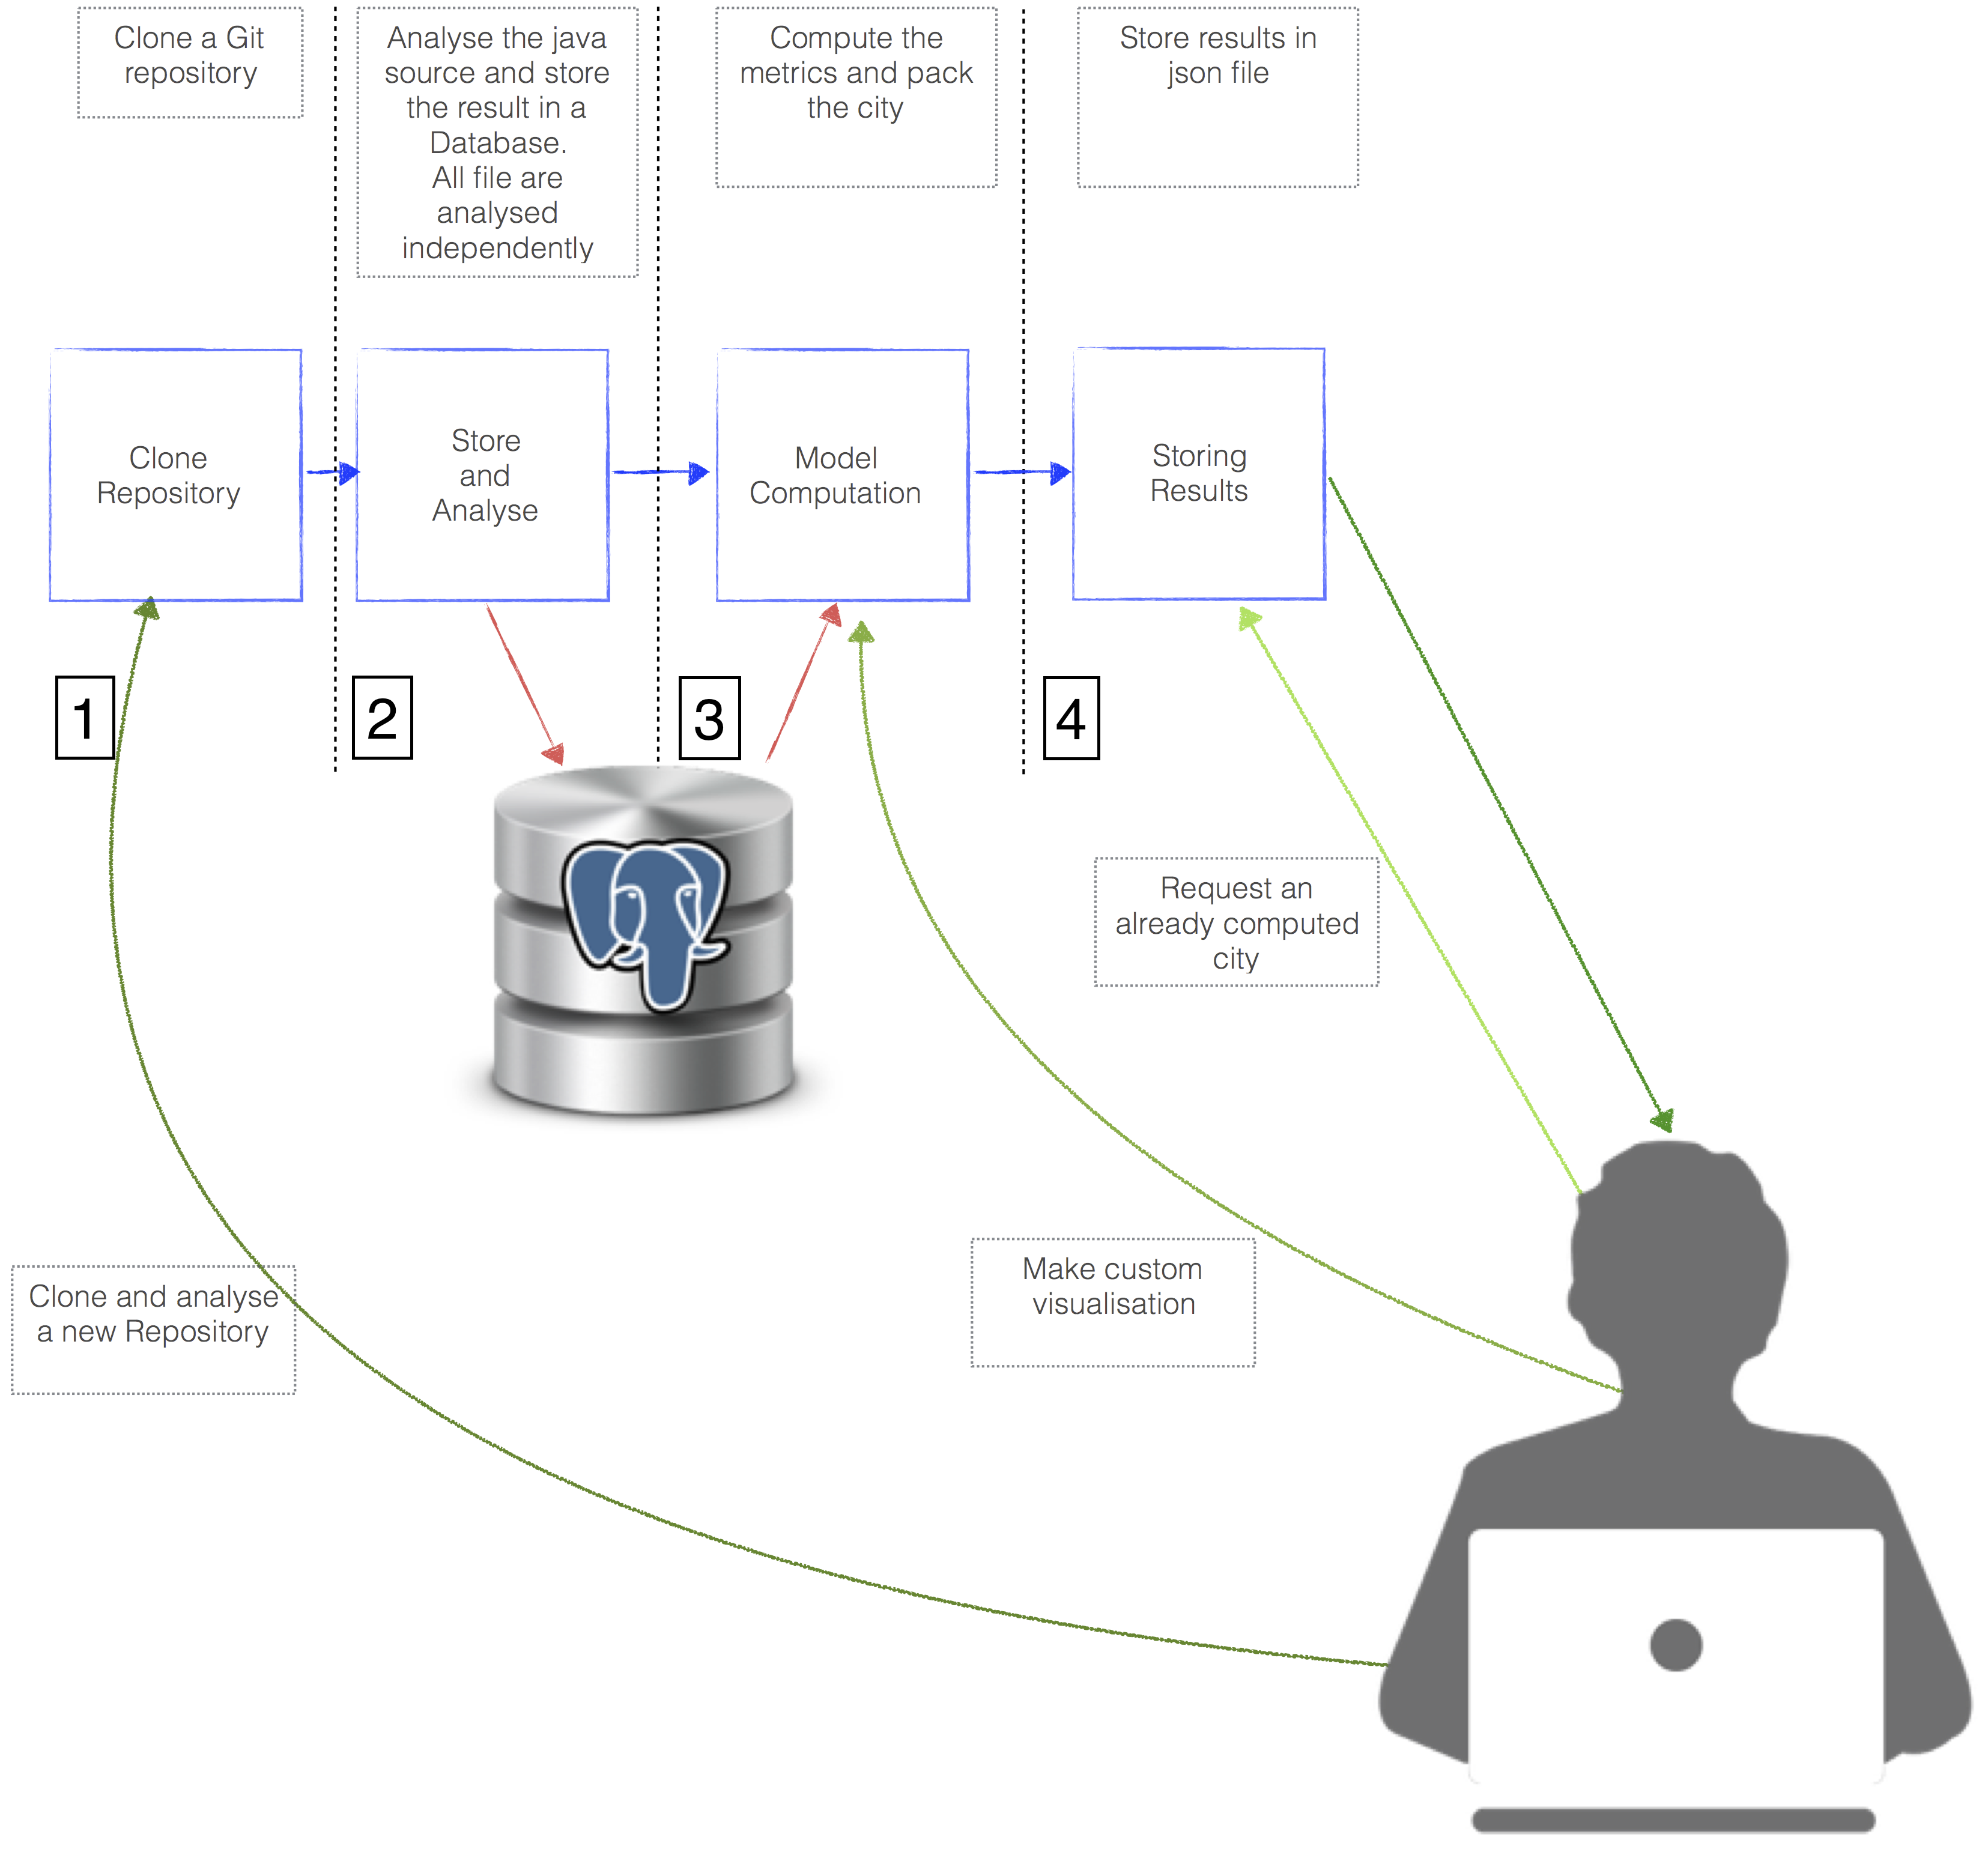
\includegraphics[width=0.8\textwidth]{images/processPipeline}
	
	\caption[Process Pipeline]{Process Pipeline\label{fig:processPipeline}}

\end{figure}

The Visualiser is the core of the system. Since is a web application, it consist in back end and a front end. All the computation are done in server side, since the amount of data is big, we also adopt a strategy to precompute the main metrics and store it a Json file.\\
To get a better understanding how the system works we can use an example. The first thing to do is upload a repository. We using a git subversion system, so the only thinks you have to do is write the url of your git repository, select the user password if is needed. At this stage the system stat cloning your repository.When the the repository is cloned, it start to analyse the files, this process simply traverse the directory of the the repository and, if a java file is found, it made a AST over that file. This process write on the database all the file characteristics. \\

The next stage  start compute the cities. Since the project structure is a tree we maintain this structure during all the process. To improve the performance during the visualisation, we generate one city for each different metric computation. All the action apply on this stage are like  functions apply to each node a the tree. The first pass throw the tree is the size computation, that give to each node the metrics result for width, height and colour. The next pass set the colour. What we are doing is to map the metrics colour value in a range 0-1. The rendering in client side set the real colour from light blue to purple. After we also compute the package colour and at the end we pack the city.\\
The packing algorithm is dome as if each package reside in the origin. Only during the rendering time we move the package around the scene.At the end we store the result in a json file. This file contains a tree whit all the information.\\
We gives also the opportunity to the user to make his own city, by deciding through a predefine list of metrics to assign to each  dimension. This process does exactly the same thing as done after the AST.\\

The front end part gives to the user a way to interact whit the system. The most interesting part is the rendering of the json. You could imagine this process as draw each block on the origin and when the parent is drawn we move his children from the origin to the correct position. In reality is work in the opposite way: the root is in the origin and at each recursion we assign a new origin in which the package should be drawn.We using Babylon.Js as 3d engine that works on top of webGl. Since we are on a browser you can not have more then 10k of boxes. The shader apply to each block is a easy implementation  of Cel Shading , but since we can not apply two passes for each frame and we have simple box, we used a faster version that still has a good effect without affect performance. Easily using the UVs of the texture and the actual size of each box. If you use the same shader with circle or anything else it doesn't works.\\

We also implement a small query system that gives a way to search file or package on the city. By double clicking on a building it appear a pop up whit the java code and we highlight the key word to made the code readable. Also there are a list of discussion views.\\ 



   





\newpage
\section{Evaluation} \label{evaluation}

\subsection{Introduction}
In this section we are going to analyse two project by using our tool. 
The analysis of this project is split in two parts. The former part speak about the structure, we are looking  for code identity harmony see \ref{sec:idHarmony}. The latter part we are going to analyse the information cover. 
For the former part we can't say that a particular design is wrong, we could only give a monitor to the developer to check some port and understand if it's correct.
You can navigate and play with this two project on \url{http://rio.inf.usi.ch:51001/}. 

\subsection{Tomcat}
The Apache Tomcat software is an open source implementation of the Java Servlet, JavaServer Pages, Java Expression Language and Java WebSocket technologies. 
The Apache Tomcat software is developed in an open and participatory environment. The Apache Tomcat project is intended to be a collaboration of the best-of-breed developers from around the world.

\subsubsection{Code related analysis}

\begin{figure}[h]
\centering
\subfigure[Tomcat: Classes ]{
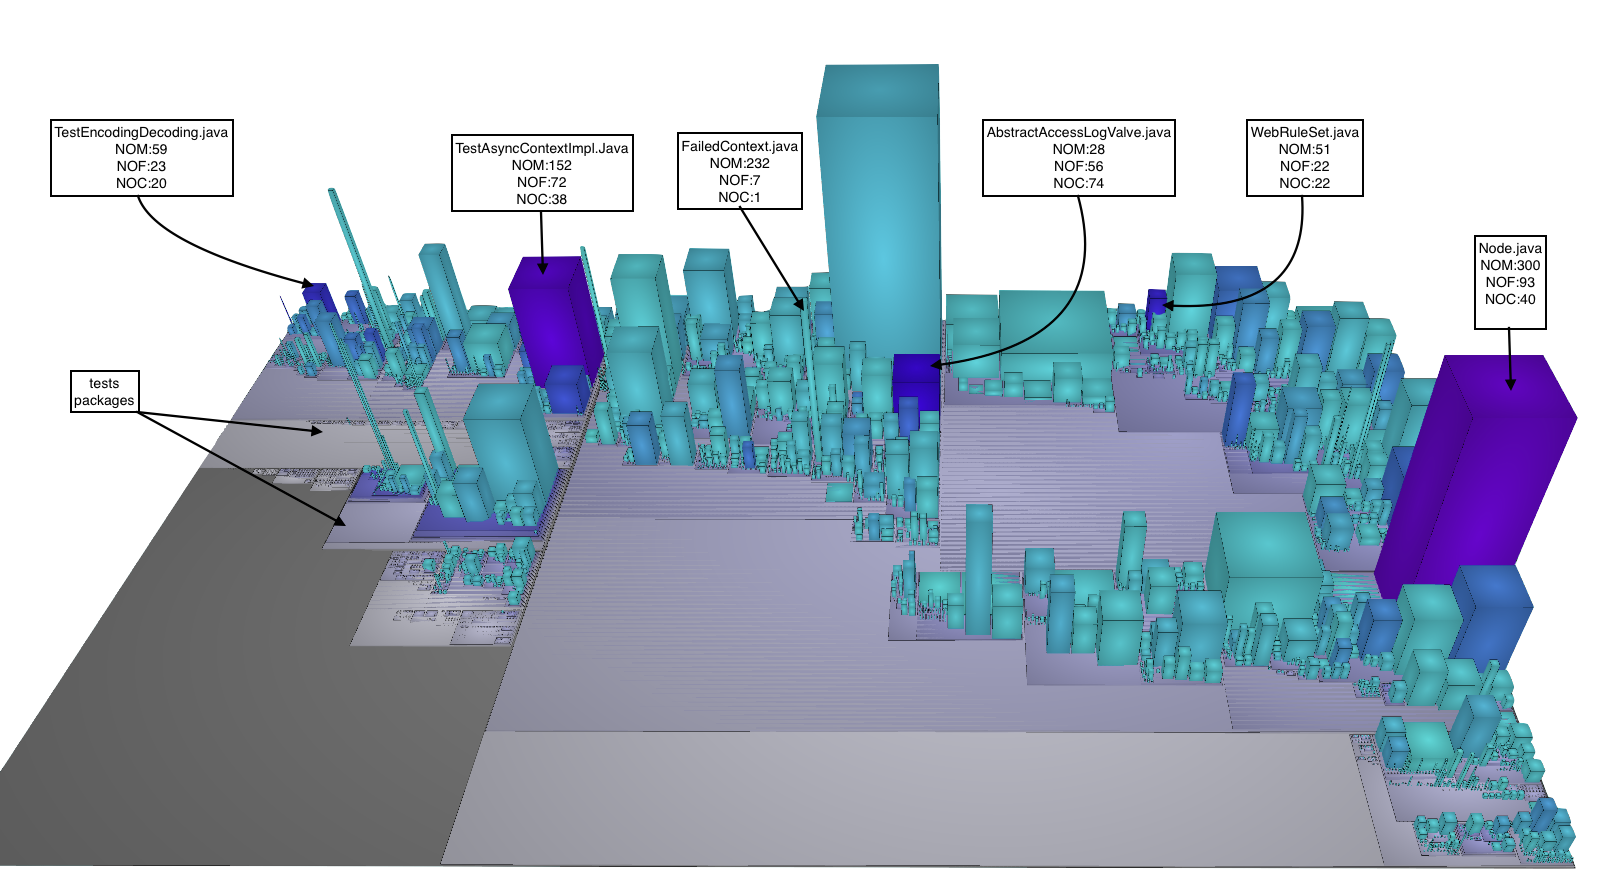
\includegraphics[width=.45\textwidth,height=4cm,keepaspectratio]{images/tomcatClss}
\label{fig:tomcat:a}
}
\hspace*{\fill}
\subfigure[Tomcat: Interfaces]{
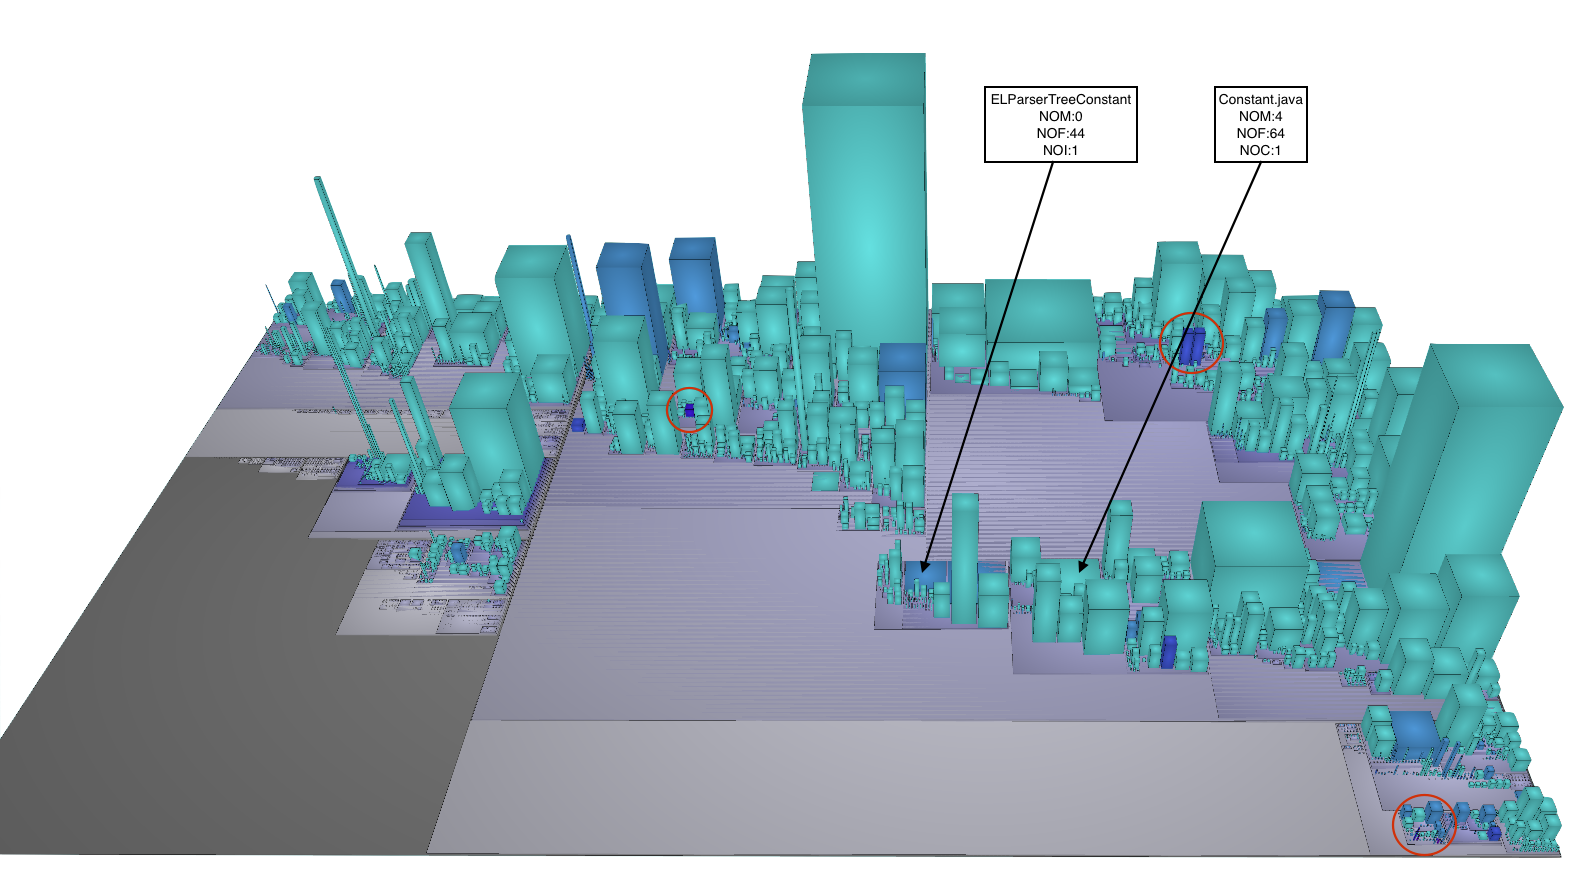
\includegraphics[width=.45\textwidth,height=4cm,keepaspectratio]{images/tomcatInt}
\label{fig:tomcat:b}
}

\hspace*{\fill}
\subfigure[Tomcat: Zoom Interfaces]{
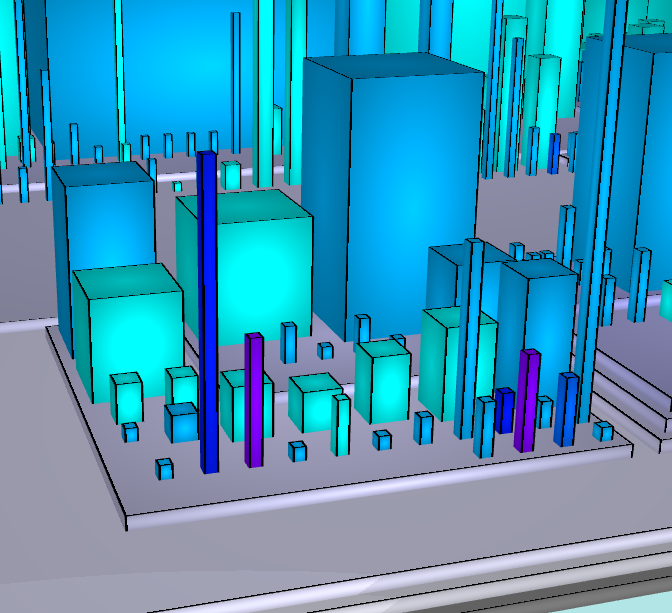
\includegraphics[width=.45\textwidth,height=4cm,keepaspectratio]{images/tomcatWInt}
\label{fig:tomcat:c}
}

\caption{Tomcat \label{fig:tomcat}
}

\end{figure}


Figure \ref{fig:tomcat} depict tomcat's code related infrormations. The building represent the java files post on top of his package. The height of a building is the number of method and the width is the number of field. The colour represent in Figure \ref{fig:tomcat:b} the number of interface and in \ref{fig:tomcat:a} the number of classes.\\ 
Generally we have an equal distribution of class and interface for each file, there are only a few anomaly. Whit this software we can not understand if this anomaly are an error or not, we can only give to the developer a monitor to check class that looks strange.\\
In Figure \ref{fig:tomcat:a} appear clear that there are some classes that has a height concentration of inner classes. Infect if you open the file you'll see a huge number of private static class. This is not a problem for the Java Code Conventions  \cite{oracle} infect there are not more then one public class and all the other inner class are inside the public class. The name and the characteristics are written on the image. As you can see, 2 of them are test classes the other 3 are not.The test class are fine.Tho other three classes could have a high level of coupling that is an hint to check the design.
Regarding the interface, we  have some  files that contains more then once. In this case we have not big number of interface so it could be a design  chose and not a problem.\\
Now we take a look on the method and fields of a class. As we can aspect the class Node.java has a lot of methods but at the same time have a huge number of classes as sow before.
It is a good candidate for a God Class. As well as Node.java also StandardContex.java has the potential to be a god class either,  since he has only thee classes and a huge number of methods and fields. In both class we can incur in a high level of coupling.\\
There are a few buildings that looks like a brain class. We don't care about test class since are, by definition a list of methods. The fist one is FailledContext.java, that as a huge amount of methods and no too much fields. As you can see from image there are other classes of this type.\\
The Data class are not too much, once is call,  Constant.java and there are others on the figure \ref{fig:tomcat:b}.



\subsubsection{Corollary Information analysis}
\begin{figure}[h]
\subfigure[Tomcat: Discussions ]{
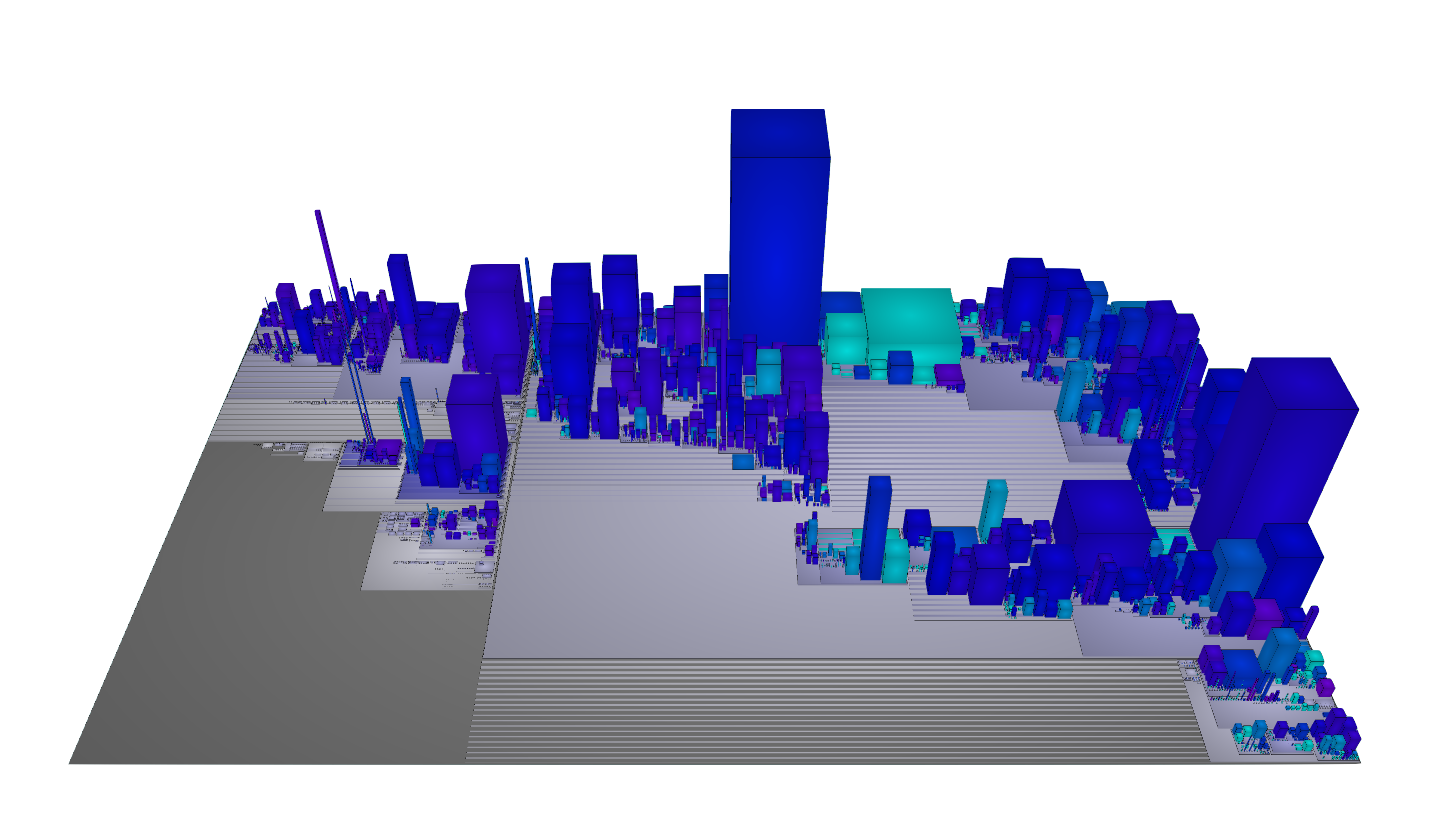
\includegraphics[width=.45\textwidth,height=4cm,keepaspectratio]{images/discussionTomcat}
\label{fig:tomcatCorrollary:a}
}
\hspace*{\fill}
\subfigure[Tomcat: Java Documentation]{
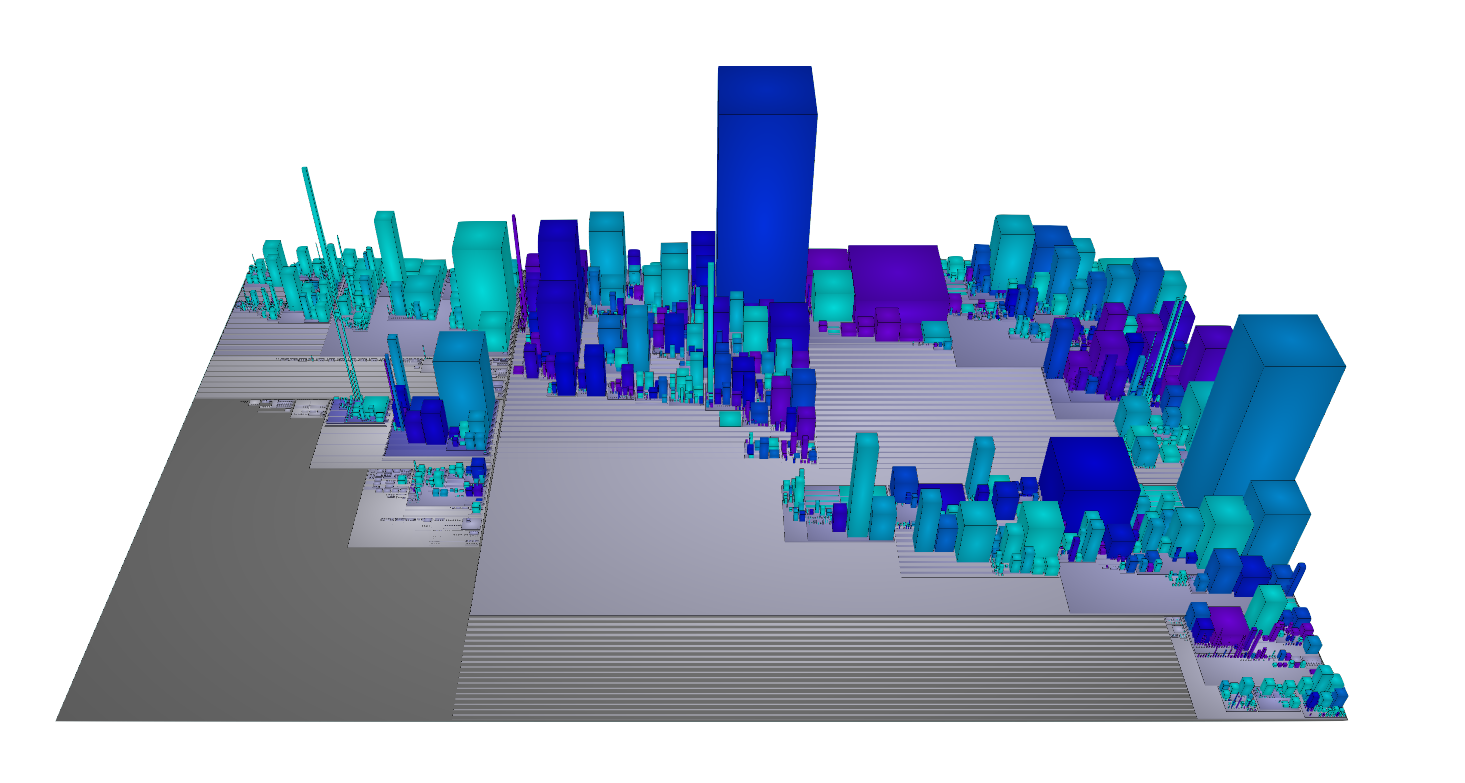
\includegraphics[width=.45\textwidth,height=4cm,keepaspectratio]{images/javadocTomcat}
\label{fig:tomcatCorrollary:b}
}

\subfigure[Tomcat: Discussion and Java Doc]{
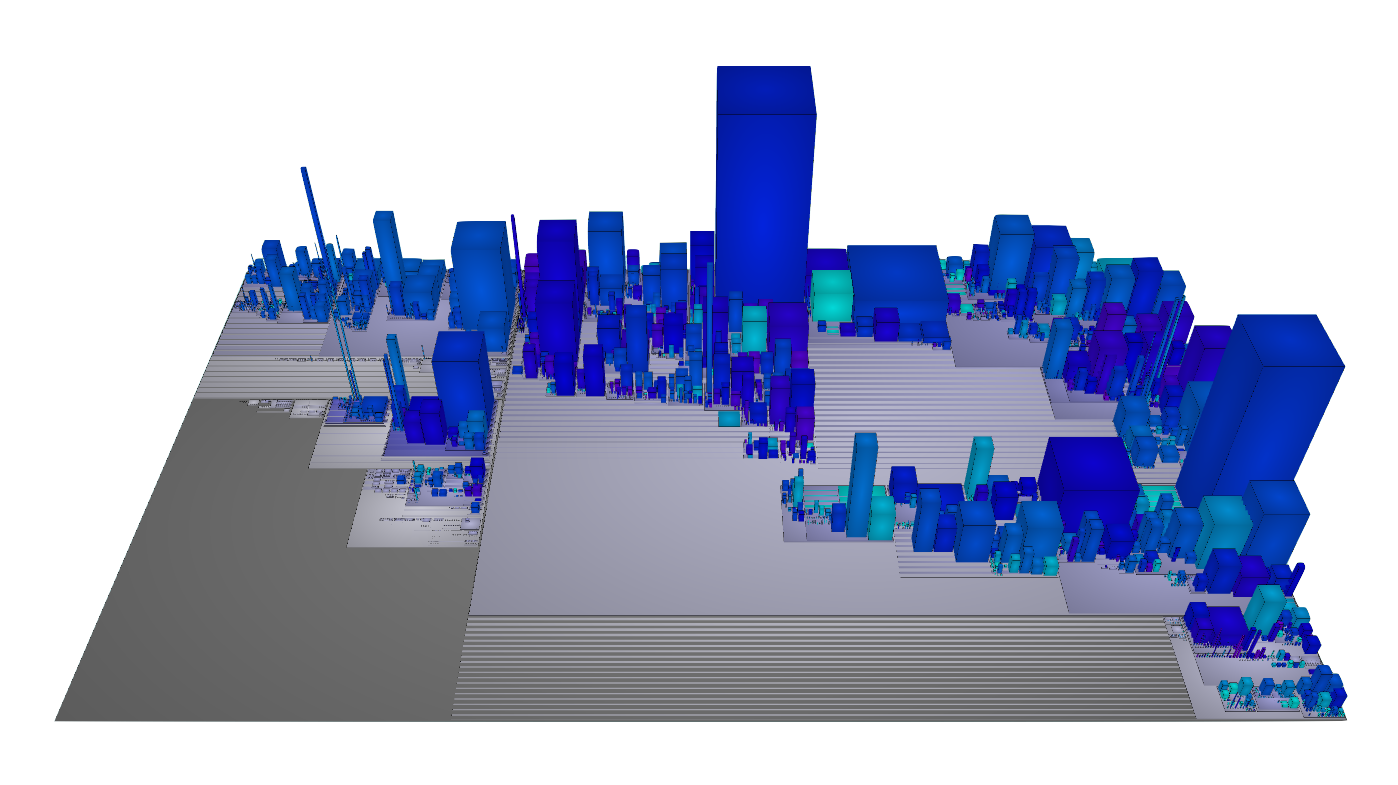
\includegraphics[width=.45\textwidth,height=4cm,keepaspectratio]{images/javaDocAndDiscussionTomcat}
\label{fig:tomcatCorrollary:c}
}

%\hspace*{\fill}
%
%\subfigure[Tomcat: Discussion and Java Doc only package ]{
%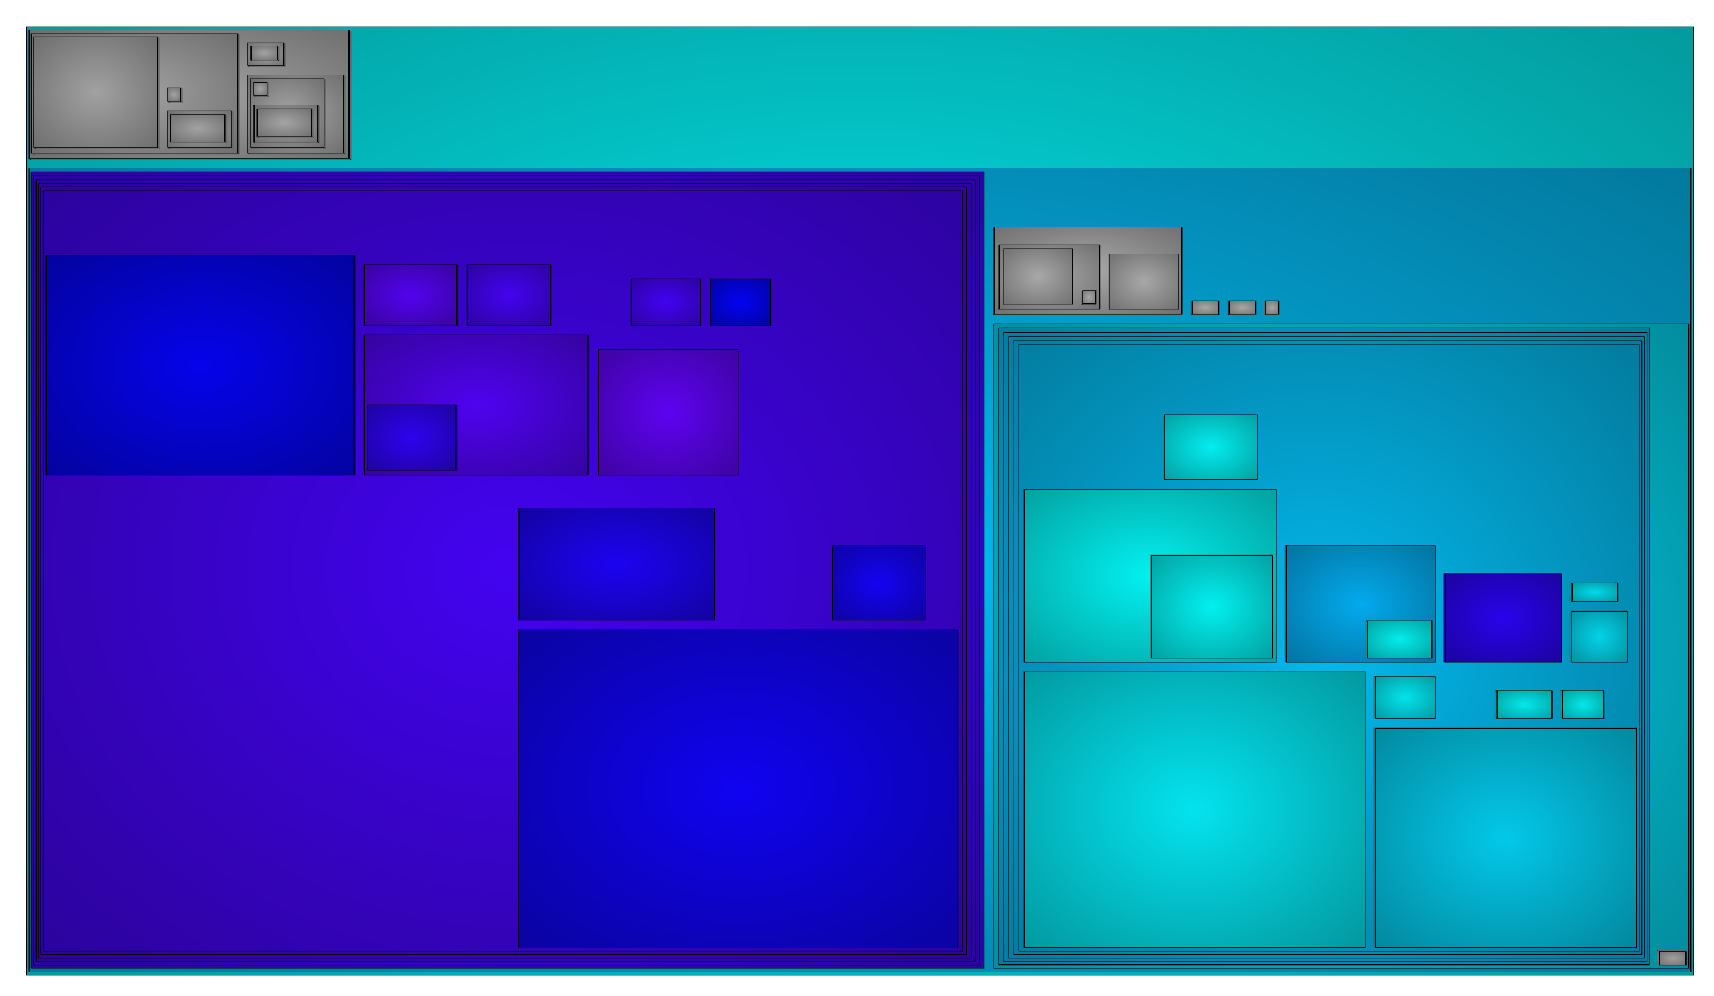
\includegraphics[width=.45\textwidth,height=4cm,keepaspectratio]{images/javaDocOnlyPackage}
%\label{fig:tomcatCorrollary:d}
%}

\caption{Tomcat Corollary Informations \label{fig:tomcatCorrollary}
}
\end{figure}
Figure \ref{fig:tomcatCorrollary} depict tomcat's code corollary  informations.The building represent the java files post on top of his package. The height of a building is the number of method and the width is the number of field. The colour represent in Figure \ref{fig:tomcatCorrollary:a} the number of discussion over methods, in \ref{fig:tomcatCorrollary:b} the number of java documentation over methods and  in \ref{fig:tomcatCorrollary:b} the information coverage.\\
Let's start analysed the java documentation:  is possible to see there are classes completely documented and others that has not documentation at all. The tests are completely not documented and some of the class that as more methods has a lower percentage of documentation, this is bad.\\
Instead the discussion coverage is pretty good. The colour of the city in average is dark blue and there are a lot of building purple.\\
Now that we have the result of both metrics we can merge it together an we have the  \ref{fig:tomcatCorrollary:c}. Thanks to the discussion found online and the documentation, in general, the source code should not be too hard to understanding it.
 

 

\newpage
\subsection{JGit}
Jgit is an implementation of the Git version control system for java.We analyse the system in the same way as Tomcat.
\subsubsection{Code related analysis}


\begin{figure}[h]
\subfigure[JGit: Classes ]{
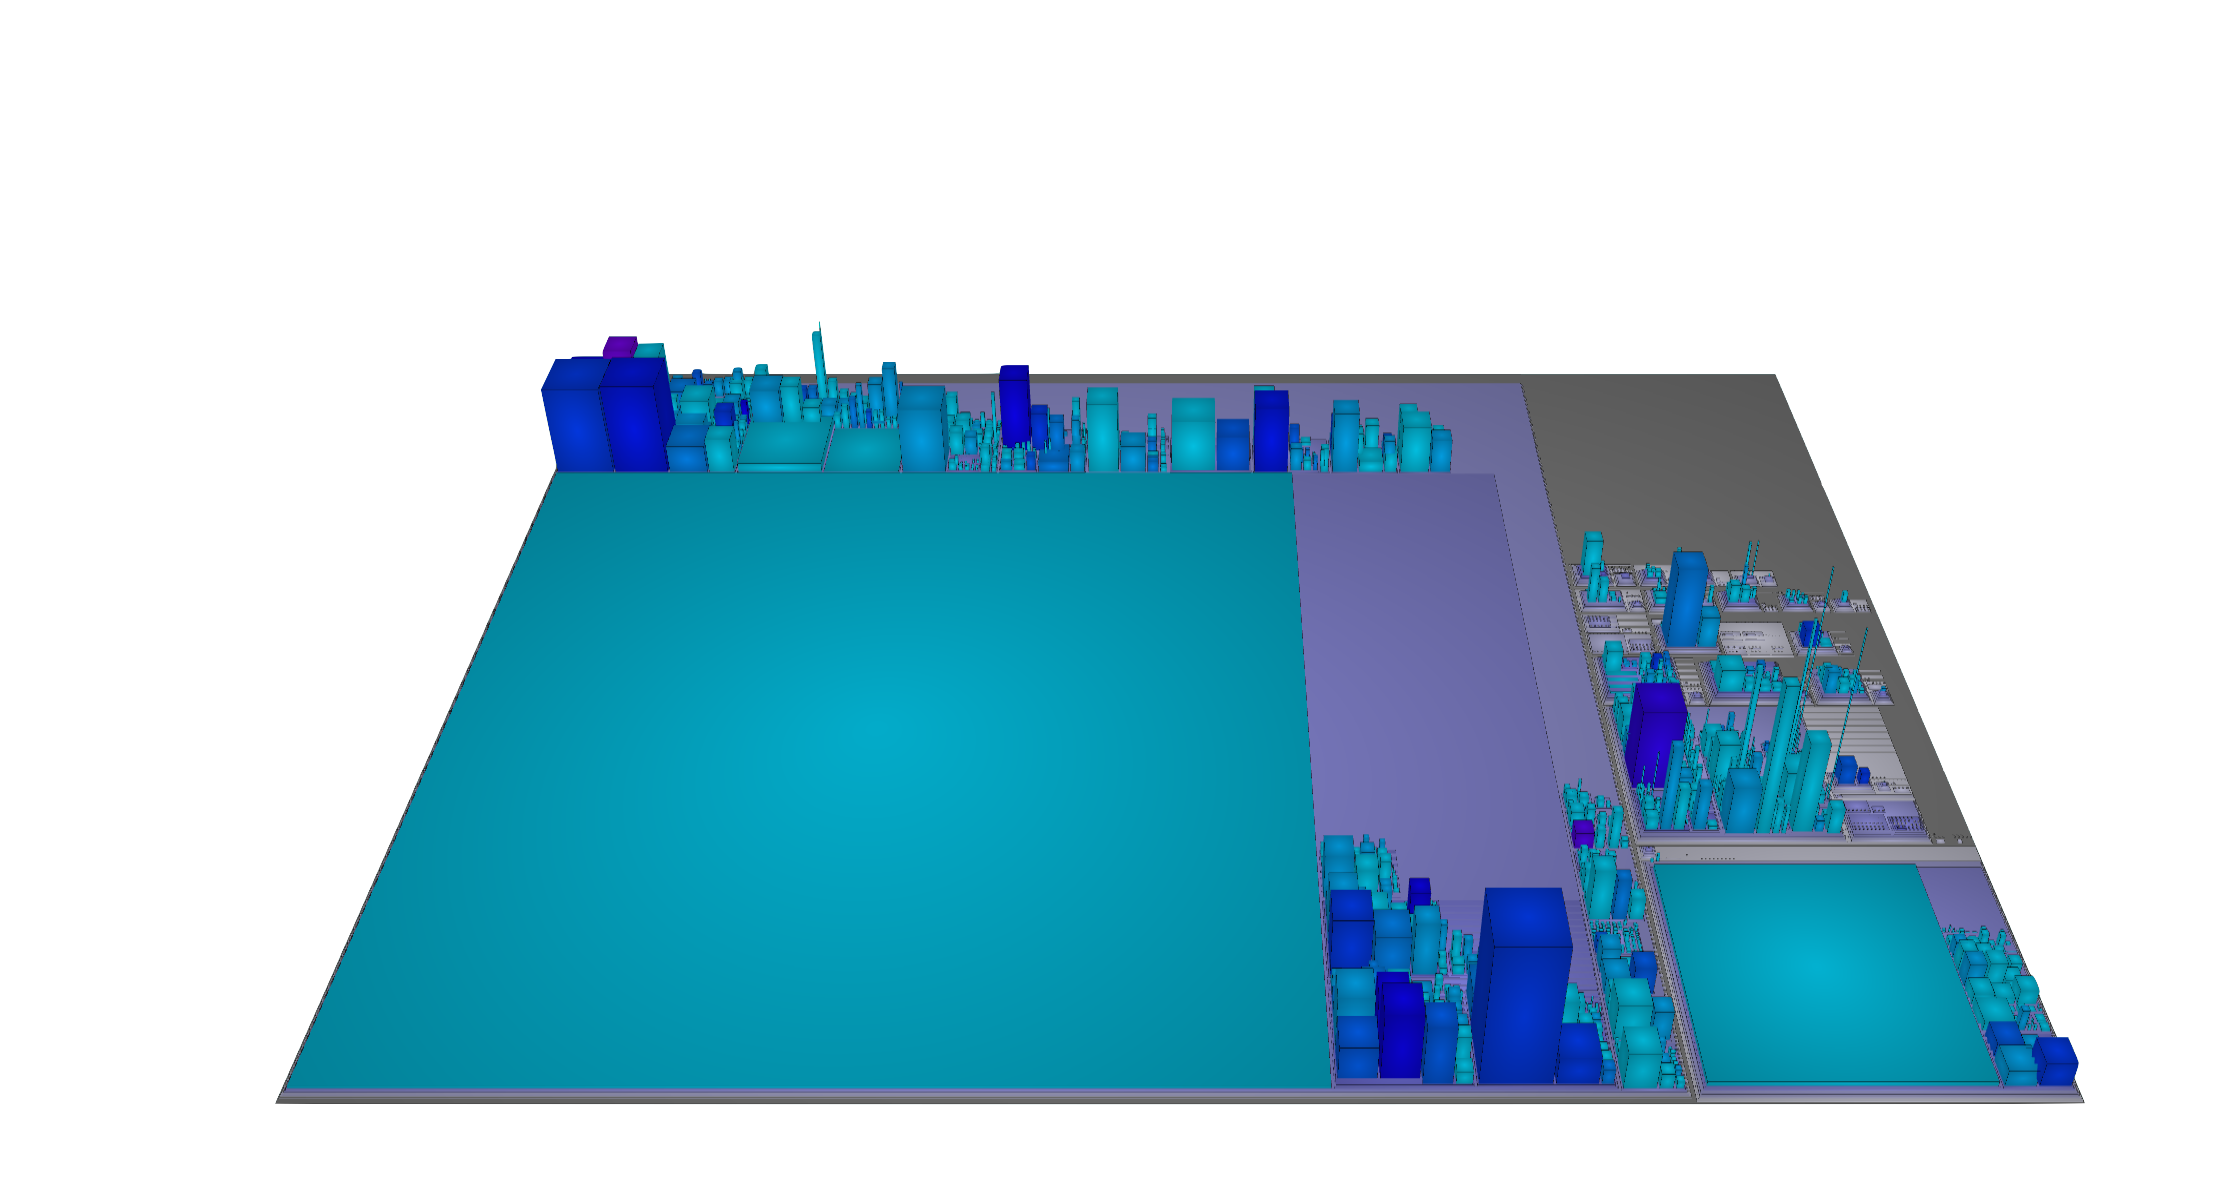
\includegraphics[width=.45\textwidth,height=4cm,keepaspectratio]{images/jgitClass}
\label{fig:jgitRel:a}
}
\hspace*{\fill}
\subfigure[Jgit: Java Interfaces]{
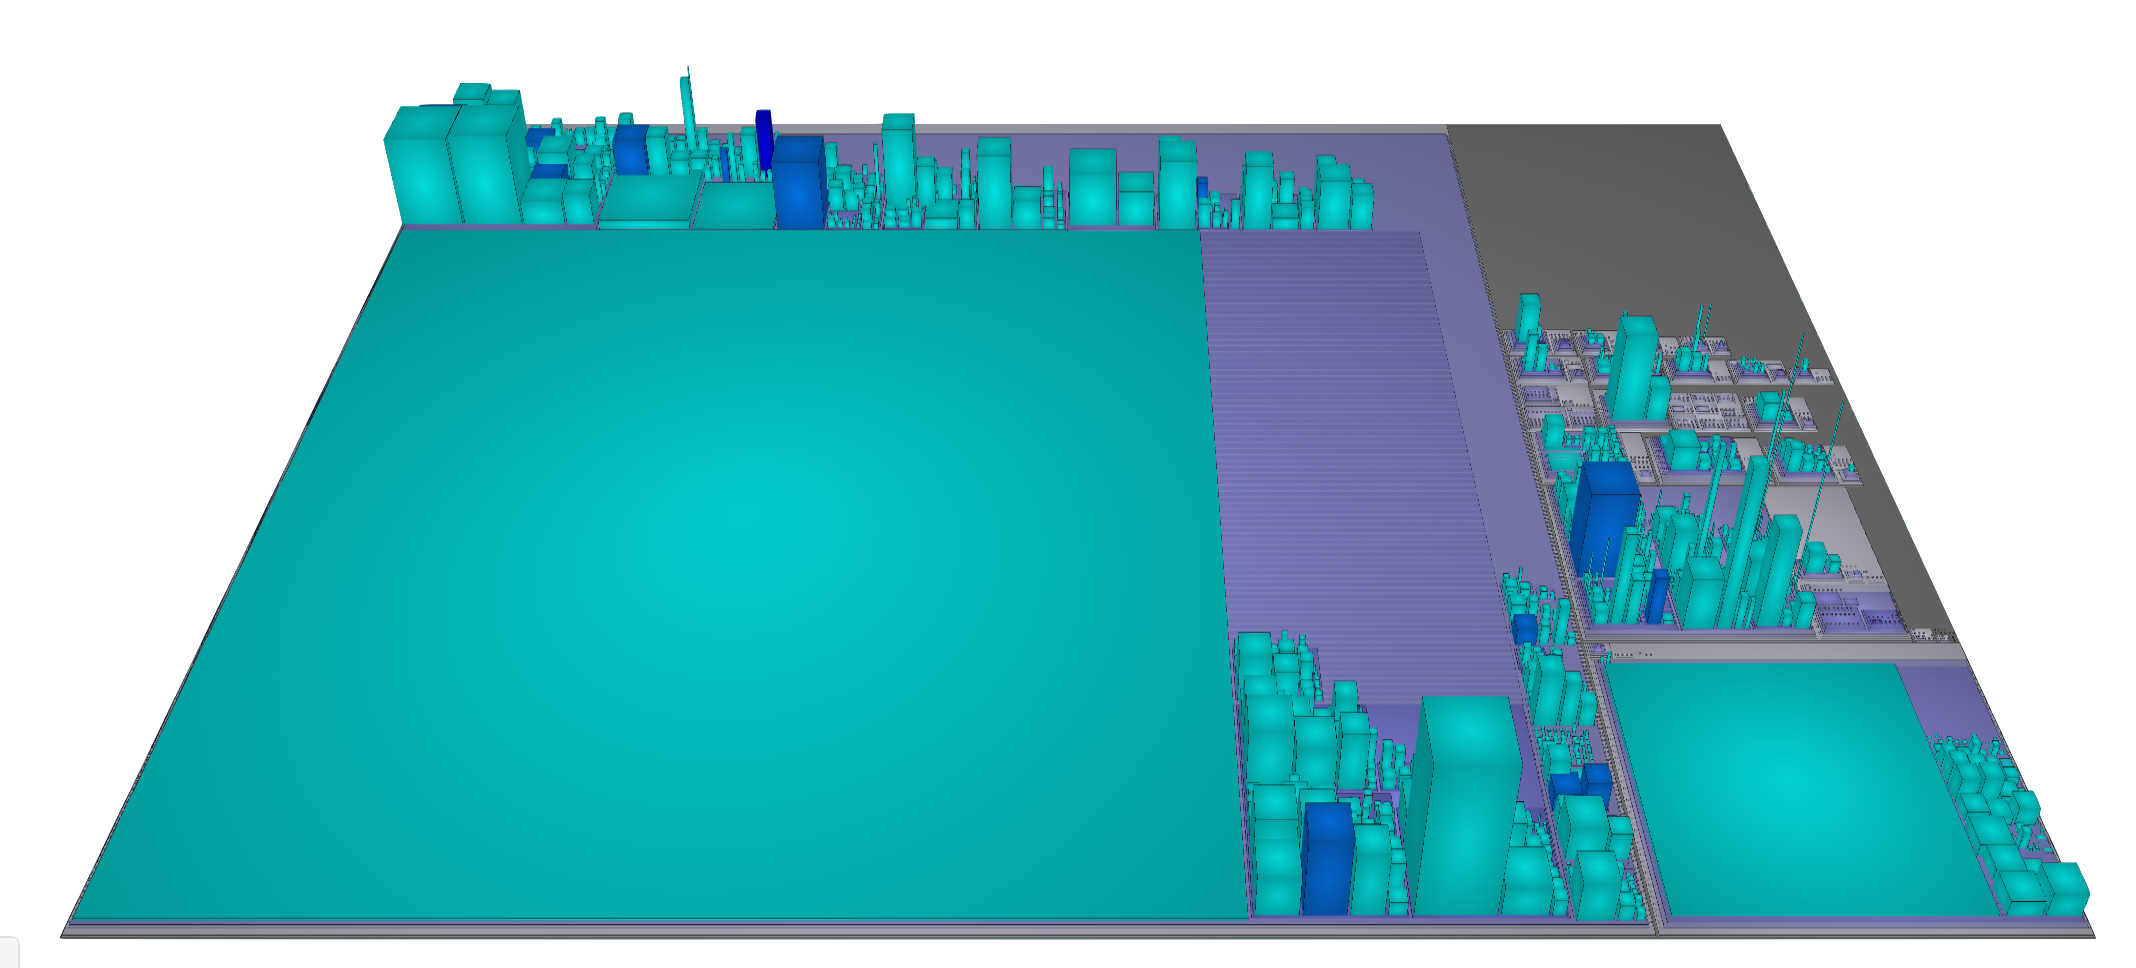
\includegraphics[width=.45\textwidth,height=4cm,keepaspectratio]{images/jgitInterface}
\label{fig:jgitRel:b}
}


\caption{Jgit Code Related Informations \label{fig:jgitRel}
}
\end{figure}

Figure \ref{fig:jgitRel} depict jgit's code related  informations.The building represent the java files post on top of his package. The height of a building is the number of method and the width is the number of field. The colour represent in Figure \ref{fig:jgitRel:a} the number of classes, in \ref{fig:jgitRel:c} the number of java interfaces.\\
The class number view shows that there are some files that have more then one class. Is important to note that the maximum amount of class is 10. Also the interface distribution appear to be well spread, there are only a few occurrence of multiple interface on the same class. Just remind that is not a crime to have more interface or class in the same file. The problem is that if you have too much you could have a small coupling degree that is bad! \\
Regarding the methods and  fields. Differently as aspected the file that has more class has not more field and methods.We can see a god class call PackWriter.java that has 48 fields and 121 methods. There are also 2 big data class:CLIText and JGitText. At last but not least there is a brain class call RepositoryState.java that has 90 methods.
 


 \subsubsection{Corollary Information analysis}
\begin{figure}[h]
\subfigure[JGit: Discussions ]{
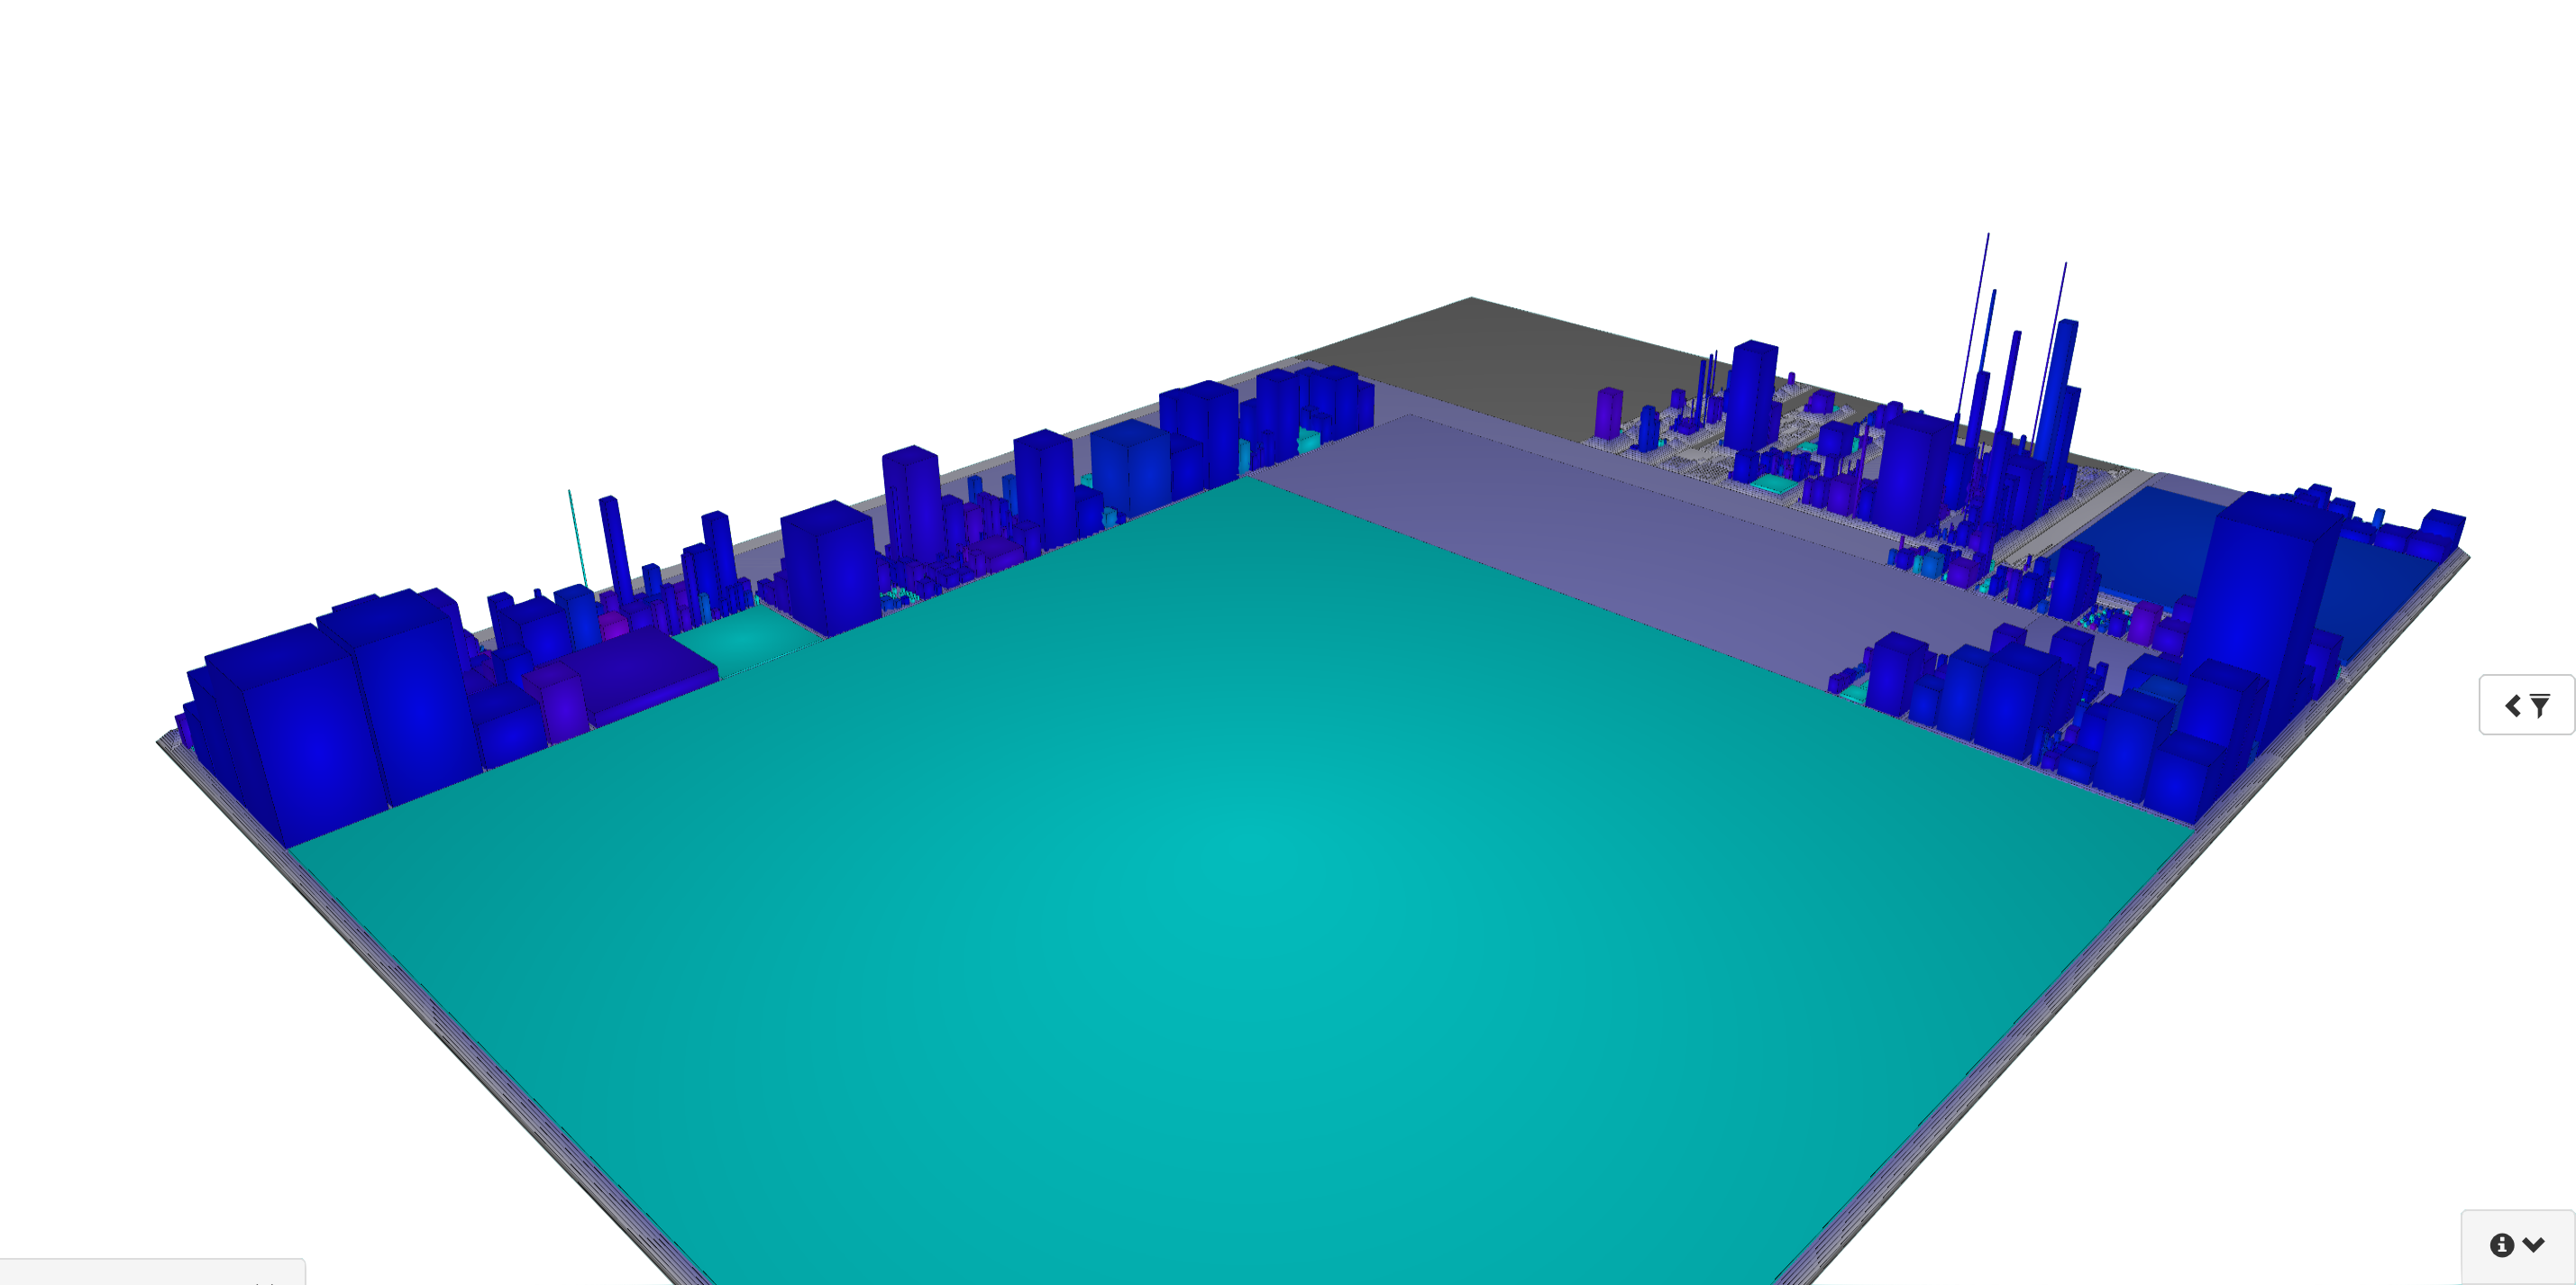
\includegraphics[width=.45\textwidth,height=4cm,keepaspectratio]{images/jgitDiscussion}
\label{fig:jgitCorrollary:a}
}
\hspace*{\fill}
\subfigure[JGit: Java Documentation]{
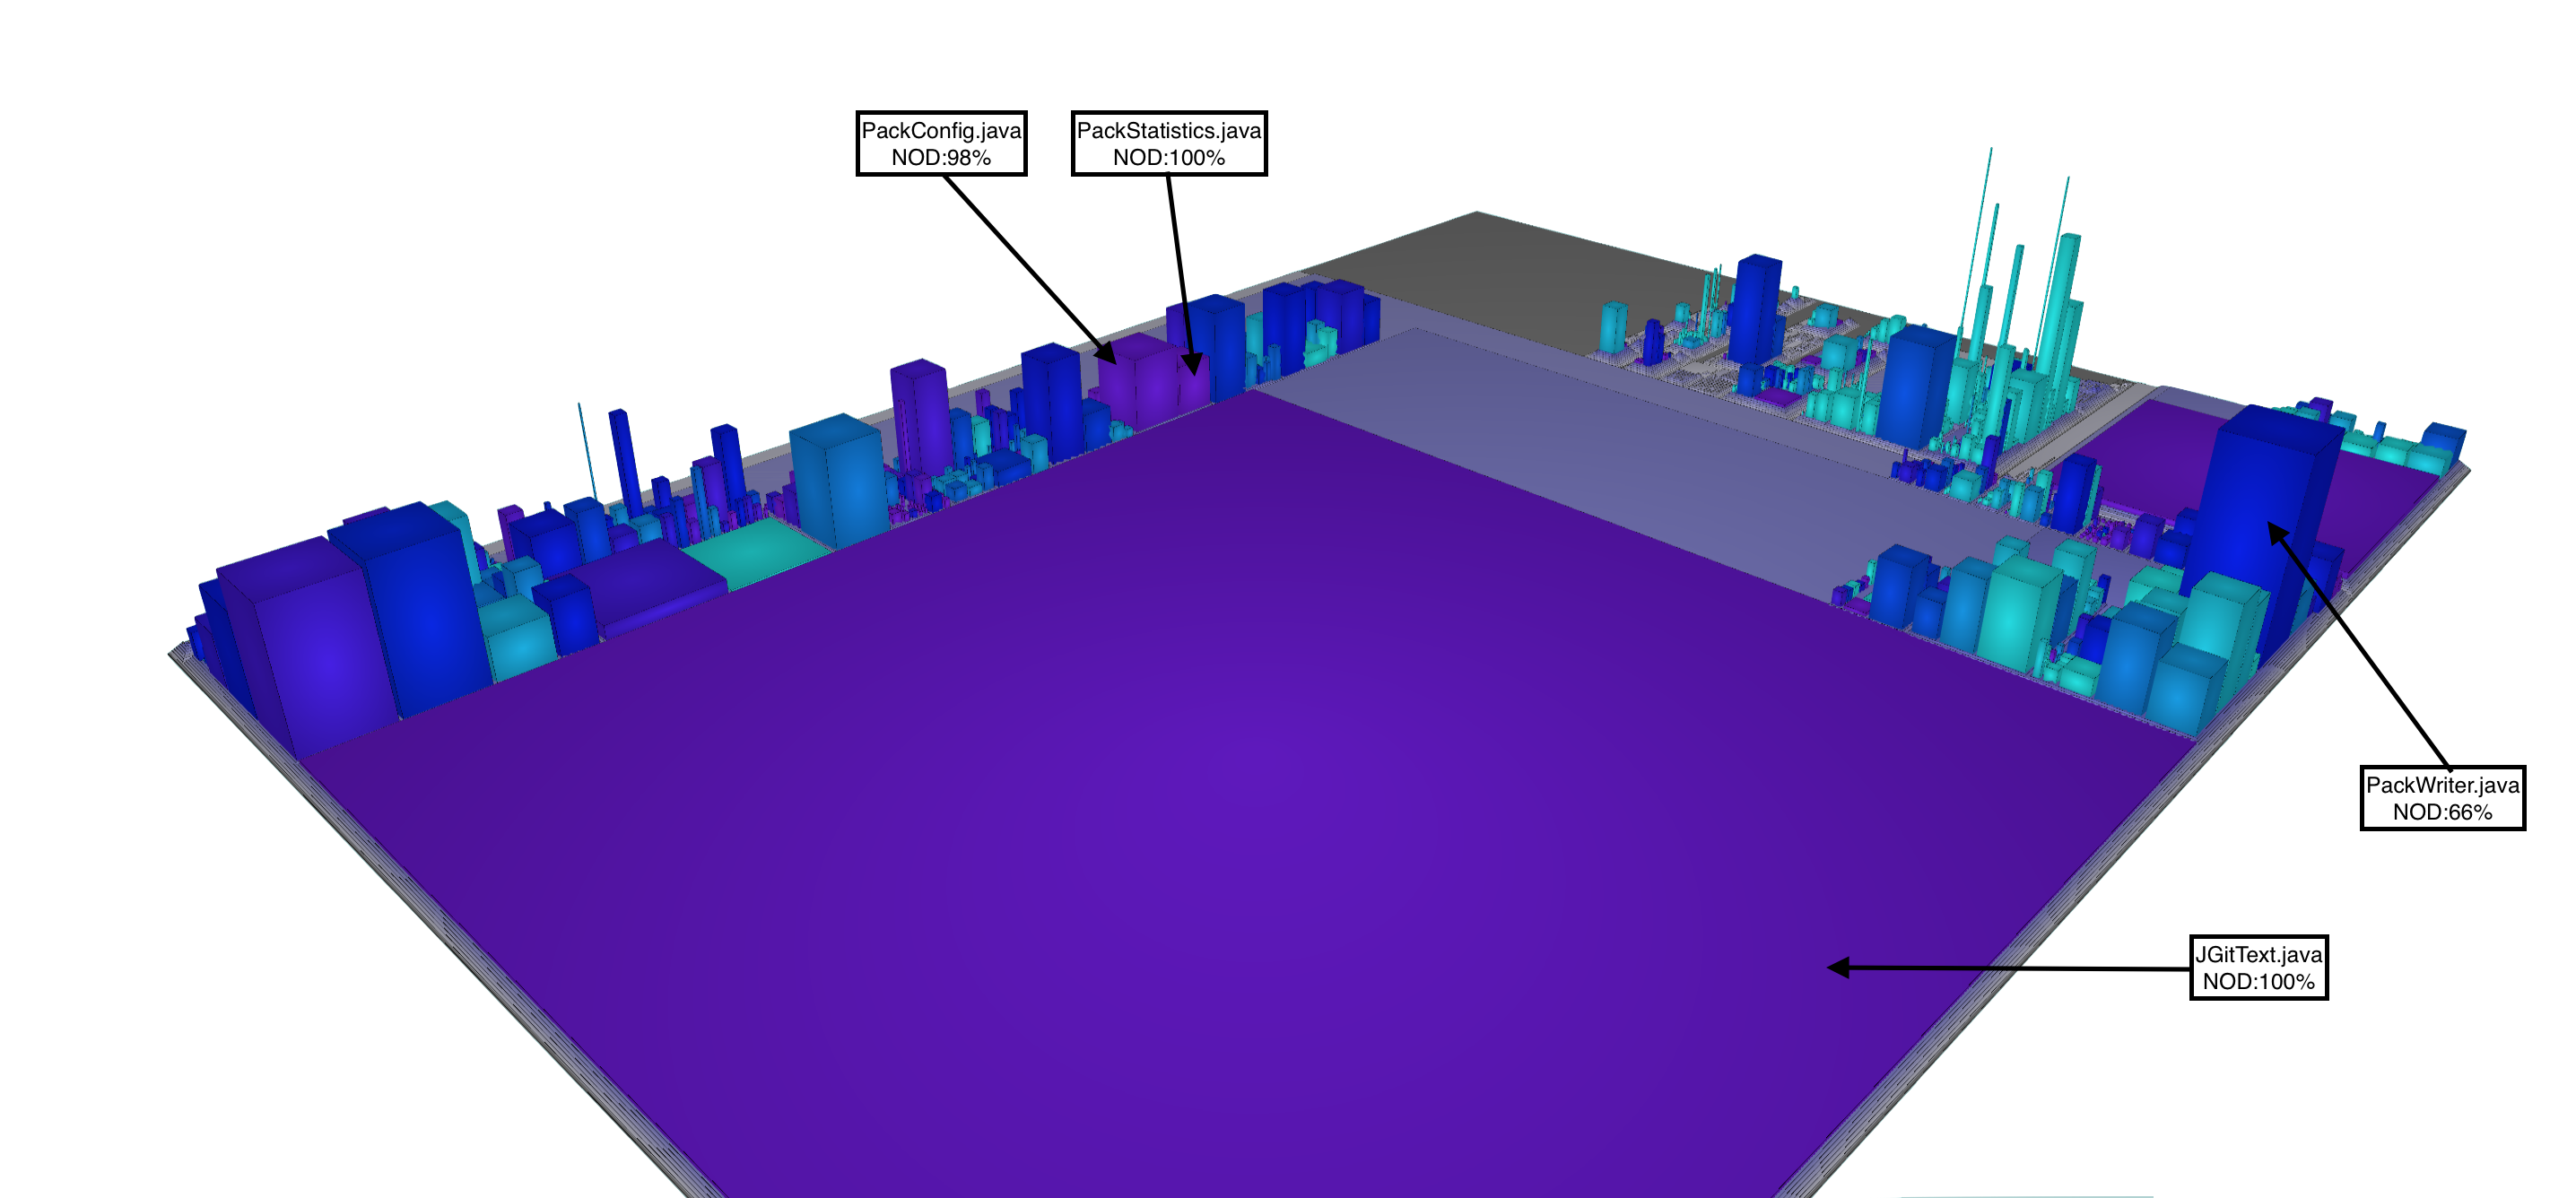
\includegraphics[width=.45\textwidth,height=4cm,keepaspectratio]{images/jgitJavaDoc}
\label{fig:jgitCorrollary:b}
}

\subfigure[JGit: Discussion and Java Doc]{
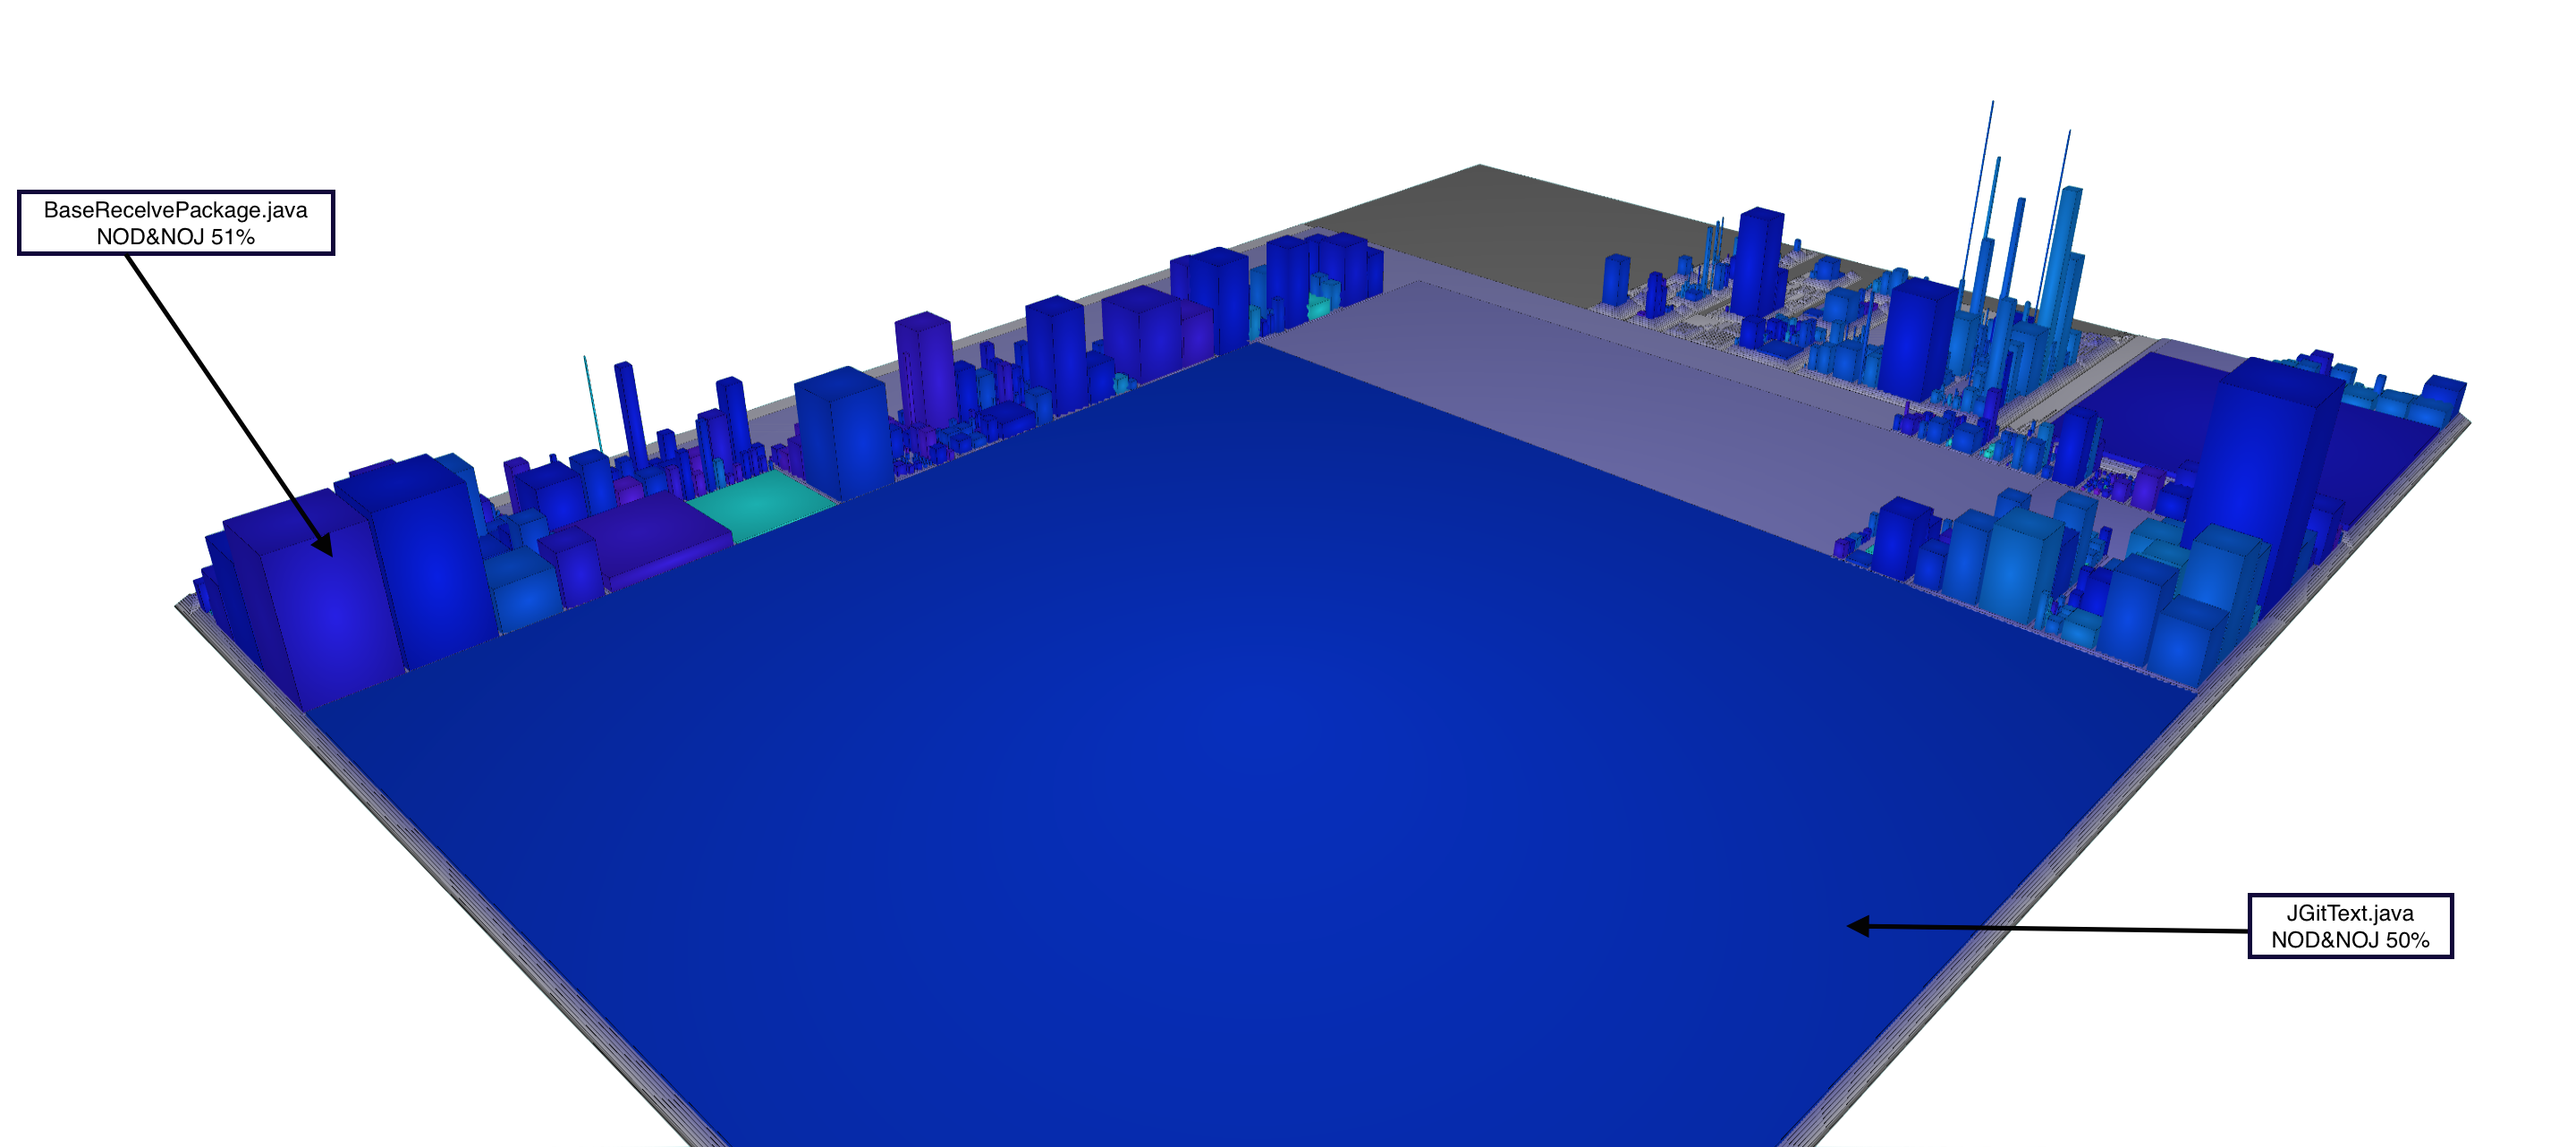
\includegraphics[width=.45\textwidth,height=4cm,keepaspectratio]{images/jgitDocDisc}
\label{fig:jgitCorrollary:c}
}

%\hspace*{\fill}
%
%\subfigure[Tomcat: Discussion and Java Doc only package ]{
%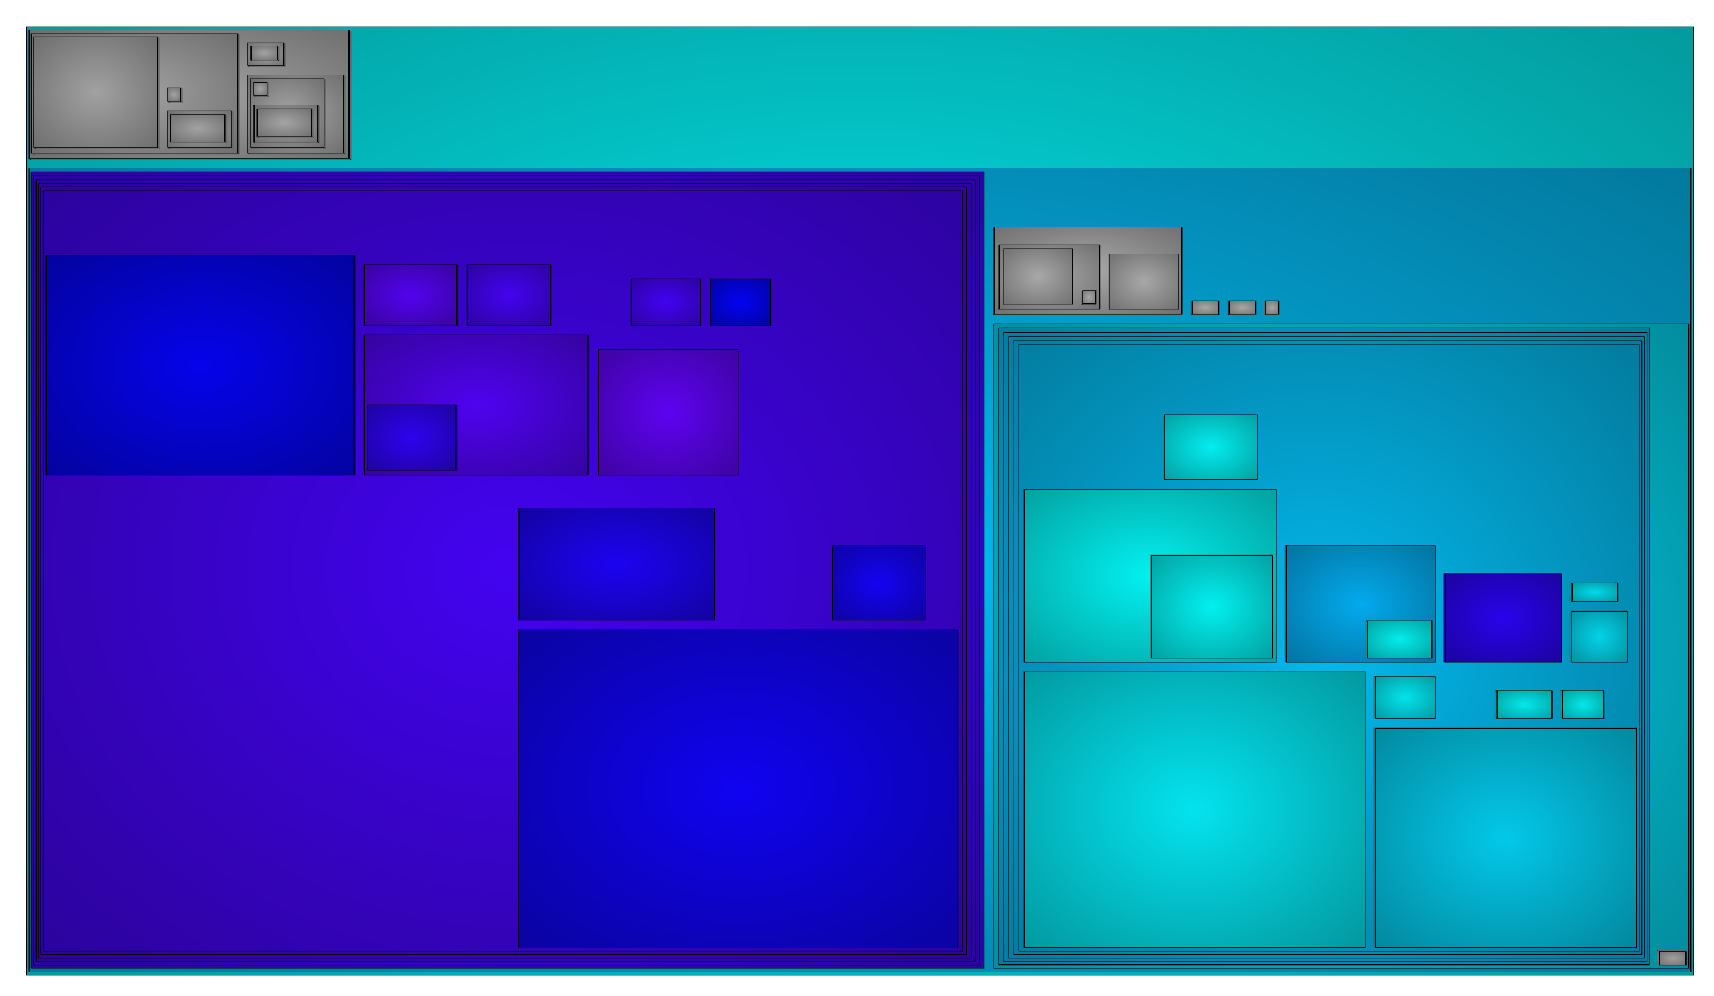
\includegraphics[width=.45\textwidth,height=4cm,keepaspectratio]{images/javaDocOnlyPackage}
%\label{fig:tomcatCorrollary:d}
%}

\caption{JGit Corollary Informations \label{fig:jgitCorrollary}
}
\end{figure}


Figure \ref{fig:jgitCorrollary} depict tomcat's code corollary  informations.The building represent the java files post on top of his package. The height of a building is the number of method and the width is the number of field. The colour represent in Figure \ref{fig:jgitCorrollary:a} the number of discussion over methods, in \ref{fig:jgitCorrollary:b} the number of java documentation over methods and  in \ref{fig:jgitCorrollary:c} the information coverage.\\
Starting by fig \ref{fig:jgitCorrollary:a} we see that the discussion available are a lot. There aren't any discussion for JGitText since has only fields.There are also a few classes with a 100\% of discussion coverage.\\
The java doc view shows on fig \ref{fig:jgitCorrollary:b} show that there are a lot of building without documentation. Some of them are tests,but a huge number are not so it should be improved.\\

In figure  \ref{fig:jgitCorrollary:c} is show a mix of both information. In general we achieve a good level of information of the entire system.  

\newpage
\section{Conclusion} \label{conclusion}
We present Cub8, a novel approach to extract information not strictly related to the code useful to improve the simplicity of understanding a source code. Is the combination of an augmented visualisation system using a 3d city metaphor with information that are retrieve from the web. It allows to get  an idea about the information available and interact with all the resources. Also it gives to the developer a way to analyse and find some code disharmony by changing metrics dynamically. He gives also some tools for filtering objects, showing code. For the moment support the clone of only GIT repository. \\
There are some improvement that could be interesting to be implemented like showing the system history or made the matching between java source method call and discussion method call more precise using a type resolution algorithm.\\
  
  



%%%%%%%%%%%%%%%%%%%%%%%%%

%\subsection{General issues}
%
%Latex is not so complex. If you aren't familiar with it just spend some time in googling for latex commands (e.g. font formats, tables, figures, items,\dots).
%
%\subsection{Getting started}
%In order to use the bachelor thesis template, be sure that the following files are present in your working directory:
%\begin{itemize}
%\item usiinfbachelorproject.cls (The latex template)
%\item logo-info.pdf (The logo figure)
%\item references.bib (The references file)\\
%\end{itemize}
%
%\subsection {Compilation issues}
%
%If you are not familiar with Tex, I advise you to download TexShop for Mac OS.\\
%To include the references and display them in the final pdf, you have first to typeset this file with \textit{LaTex} (ComboBox upper left, if you use TexShop), then with \textit{BibTex} and finally again with \textit{LaTex}.\\
%In order to resolve figures/table/\dots~references you have to run 2 times the (latex) typeset.
%
%\subsection {Document structure}
%
%Some basic sections:
%\begin{itemize}
%\item Introduction (including Motivation)
%\item State of the Art
%\item Project requirements and analysis
%\item Project design (top-down)
%\item Implementation issues (bottom-up)
%\item Tests (methodology, results, comments)
%\item Conclusions and future work or possible developments
%\end{itemize} 
%
%\subsection {Some examples}
%
%\textbf{Figure ~\ref{fig:USILogo}} shows how to insert figures in the document.
%
%\begin{figure} [h]
%\centering
%
\includegraphics[width=0.5\textwidth]{logo-info.pdf}
%\caption{Caption of the figure}
%\label{fig:USILogo}
%\end{figure}
%
%\noindent\textbf{Table ~\ref{tab:numbers}} shows how to insert tables in the document.
%
%\begin{table}[h]
%\centering
%\scalebox {0.8} {
%\begin{normalsize}\begin{tabular}{l|lll}
%\textbf{Col 1} & \textbf{Col 2} & \textbf{Col 3} & \textbf{Col 4}\\
%\hline
%1 & 2 & 3 & Goofy\\
%4 & 5 & 6 & Mickey



%\end{tabular}
%\end{normalsize}
%}
%\caption{Caption of the table}
%\label{tab:numbers}
%\end{table}


%%%%%
\newpage

\bibliographystyle{abbrv}
\bibliography{references}

\end{document}